\documentclass[12pt,oneside,a4paper,english]{article}
\usepackage[T1]{fontenc}
\usepackage[latin2]{inputenc}
\usepackage[margin=2.75cm,headheight=26pt,includeheadfoot]{geometry}

\usepackage{listings}
\usepackage{color}
\usepackage{titlesec}
\usepackage{titling}
\usepackage[framed, numbered]{matlab-prettifier}
\usepackage{changepage}
\usepackage{amsmath}
\usepackage{hyperref}
\usepackage{enumitem}
\usepackage{graphicx}
\usepackage{fancyhdr}
\usepackage{lastpage}
\usepackage{caption}
\usepackage{tocloft}
\usepackage{setspace}
\usepackage{multirow}
\usepackage{titling}
\usepackage{float}
\usepackage{comment}
\usepackage{booktabs}
\usepackage{indentfirst}
\usepackage{lscape}
\usepackage[english]{babel}
\usepackage{booktabs,caption}
\usepackage[flushleft]{threeparttable}
\usepackage[english]{nomencl}
\usepackage{xcolor}
\usepackage{lipsum}

% --- set footer and header ---
\pagestyle{fancy}
\fancyhf{}

\setlength{\parindent}{2em}
\title{Thesis} % to reference as \title, don't use \maketitle
\makeatletter\let\Title\@title\makeatother

\lstset{language=Matlab,
style=Matlab-editor,
basicstyle=\normalsize\mlttfamily,
numbers=left,
numberstyle={\scriptsize\color{black}},			% size of the numbers
numbersep=0.5cm											
}

\newlist{steps}{enumerate}{1}
\setlist[steps, 1]{leftmargin=1.5cm,label = Step \arabic*:}
\renewcommand{\headrulewidth}{1pt}
\renewcommand{\footrulewidth}{1pt}

%\lhead{\Title}
\rhead{\nouppercase{\rightmark}}
\lhead{\Title}
\rfoot{
\includegraphics[height=1.25cm]{figures/root/tuc_image.png}} % right header logo
\setlength\headheight{16pt}
\setlength{\footskip}{50pt}
\lhead{\Title} %rightH title
\cfoot{\thepage}

% --- End of page settings ---



\begin{document}
\pagenumbering{roman} 

\begin{titlepage}
\begin{center}
\vspace{2cm}

% Title

\vspace{2.5cm}
{ \huge \bfseries Technical University of Crete} % title of the report
\vspace{2.5cm}


\includegraphics[width=0.2\textwidth]{figures/root/tuc.png}~\\[1cm]
\vspace{2cm}

\vspace{2cm}

% Title
\hrule
\vspace{.5cm}
{ \huge \bfseries Title\\ of the Thesis} % title of the report
\vspace{.5cm}

\hrule
\vspace{1.5cm}

\textsc{\textbf{Authors}}\\
\vspace{.5cm}
\centering

% add your name here
Kyriakos Christodoulidis\\

\vspace{4cm}

\centering \today 

\vspace{4cm}

\textsc{\textbf{Thesis Committee}}\\

\vspace{1cm}

Professor Mania Aikaterini (Supervisor)\\
Professor Chalkiadakis Georgios\\
Professor Michail G. Lagoudakis\\
\end{center}
\end{titlepage}
\newpage
\doublespacing

%\addcontentsline{toc}{section}{Abstract}
%\addcontentsline{toc}{section}{Acknowledgments}
\renewcommand{\baselinestretch}{1}\normalsize

\tableofcontents
\newpage
\listoffigures

\renewcommand{\baselinestretch}{1}\normalsize
\singlespacing
\thispagestyle{fancy} % force page style
\newpage
\pagenumbering{arabic} 
\fancyfoot[C]{Page \thepage\ of \pageref{EndOfText}}

\newpage
\addtocounter{section}{-1}
\section{Abstract}
Computerized Motion capture methods are either very expensive to acquire or of poorer quality. Thus, we propose an innovative method that will give access to everyone that has an above-average computer, to generate for free their single-person computerized motion clips.  Recently, many researchers try to use neural networks that will estimate the 3D human pose from a single video. In our approach, we decided to use two different well-known pre-trained models, the first to find the 2D pose estimation from each frame of the video, and the other to convert these 2D poses into the 3D poses. Then, we estimated the position of the human per frame, by calculating the depth of the person in the image. The combination of the 3D poses and the position is the motion data that we wanted to find. Then, by importing these data into a Skeleton that contains all the estimated bones, we can create a  Bio-vision Hierarchy (BVH) file, that can be imported into the 3D computer graphics software toolset. At this point, the generated BVH file contains noise from the neural networks, so we propose to use some digital filters that will remove this noise without affecting the motion data information. Furthermore, we converted the raw python code into a Windows Application to create a very friendly user environment. Finally, we created some functions inside this application so that the user can visually, and edit the results from the BVH files.  
\addtocounter{section}{-1}
\newpage
\section{Acknowledgments}
First and foremost, I would like to thank my supervisor, Prof. Aikaterini Mania for her guidance and her fast response as well as her willingness to support me during my thesis. I am also grateful to Giariskanis Fotios as well as all the surreal team for their support and ideas since without them the implementation would be poorer. \\

Furthermore, I would like to thank Prof. Chalkiadakis Georgios and Prof. Michail G. Lagoudakis for their time and support to the thesis committee. I also wanted to thank Prof. Apostolos Dollas, Prof. Michalis Zervakis, and Prof. Athanasios Liavas for their advice and recommendations during my graduate applications. \\

Finally, I would like to thank my family, friends, and my colleague for the support that they gave me during my thesis.  

\newpage
\section*{Chapter 1 \\}
\section{Introduction}
\subsection{The increased demand of mocap clips}
Motion Capture (MoCap) is a cutting-edge method of capturing all or part of an actor's performance so that it can be translated into the action of a computer generated 3D character on screen. More specifically, the exact movements of the actor are captured and rendered onto the digital character. 

In the last years, there is a growing demand for MoCap in many fields including interactive virtual reality, film production, animation and so forth \cite{Efficient Content-Based Retrieval of Motion Capture Data}. However, capturing motions when needed is often not practical as motion capture systems are expensive and the capture processes are complex in general. It is often desirable to retrieve and reuse motion clips that have been captured before and stored in databases. Straightforwardly, the retrieval may be done based on text labels of motion clips. 

Therefore, using MoCap clips for production consists of the following problems. Firstly, there are a limited amount of MoCap clips that can be used and using something more unique means that the production must have the budget and the time to support it. Secondly, the majority of the stored databases of MoCap are not free to use or have poor quality.
 
\subsection{Thesis aim}
A new approach to resolving these issues is to address the problem with Neural Networks. More specifically, in this thesis, we propose a composition of a deep neural network \cite{Exploiting temporal information for 3D pose estimation} that will estimate the 3D human pose, and the output of the DNN will be saved into a Bio-vision Hierarchy (BVH) file. The task is to predict a pose skeleton for the person in each image of a video. Currently, human pose estimation is one of the challenging fields of study in computer vision which aims in determining the position or spatial location of body keypoints (parts/joints) of a person from a given image or video. 

The first step is to use a pre-trained deep neural network that can estimate these 2D keypoints. Afterward, \cite{3D Human Pose Estimation from Deep Multi-View 2D Pose,3D Human Pose Estimation Using Convolutional Neural Networks with 2D Pose Information} in order to achieve our goal we will use another pretrain model that will be fed with a 2D pose estimation as the input, estimates the 3D pose. However, estimating a 3D human pose from a single image is more challenging than 2D cases due to the lack of depth information, so the accuracy drops significantly. In order to increase the quality of the estimation, we suggest using the butter-worth filter, which removes noise from data without affecting the motion. After obtaining the smoothed 3D human pose, we need to create a skeleton, based on the joints that the first model estimated and import the keypoints to each corresponding bone. Finally, the BVH file will be created and it can be further cleaned manually by an animator in any 3D computer graphics software (Blender, Maya, AutoDesk). 

However, the code implementation will be in python, and most animators may struggle to install and run the code. In order to avoid this issue, we developed a Windows Application, that anyone can use that runs the python code of the Thesis.  
\subsection{Thesis Structure}
This thesis is organized in 6 Chapters:

	\begin{itemize}
		\item Chapter 1\\\\
            In this Chapter we discuss about the problems of the MoCap clips production and propose a solution to it. 
		\item Chapter 2\\\\
            In this Chapter, we provide the reader with a overview of some knowledge about MoCap Clips, as well as some pioneer studies and state the novelties of this study. Then, we present an approach with Generative Adversarial Networks (GAN's) that was a possible solution of the problematic situation, and the reasons that we aborted this solution.
		\item Chapter 3\\\\
		    In this Chapter, we show the reader the minimum requirements of the hardware that the proposed DNN needs in order to run. In addition, we suggest to the users the best case scenarios of the input, in order to improve the algorithm estimation. Finally, we present the Interface of the Windows Application UI.  
		\item Chapter 4\\\\
            In this Chapter, we explain the implementation of the algorithm as well as some important knowledge that is covered in the thesis. More specifically, the reader will be introduced to some pretrained models that are essential to the solution, and the procedure that these models use in order to estimate the orientation and location of the person. Having created the BVH file, we develop an Animator Tool, that animators can use to improve the results. Finally, we present the python library that allows us to convert the python code to a Windows Application, as well as the features of the Application. 
		\item Chapter 5\\\\
            In this Chapter, we compare the performance of the pretrained models in the ideal circumstances for each model. Moreover, we calculate the accuracy between a real and generated clip, and the reader will learn the circumstances that our model needs in order to work at its best.
		\item Chapter 6\\\\
            In this Chapter, we summarize our results and discuss our contribution. Finally, we address the disadvantages of our approach as well as some future ideas that would improve our work. 

	\end{itemize} 

\newpage
\section*{Chapter 2 \\}
\section{Background}
\subsection{Mocap clips}
Many different disciplines use motion analysis systems to capture human body movement and posture. Basic scientists want to learn more about the mechanisms that are used to translate muscular contractions about articulating joints into functional accomplishments like walking. Researchers are increasingly attempting to better understand the relationship between the human motor control system and gait dynamics.

Motion capture \cite{Review on Motion Capture Technology} is now widely used in the gaming, film, and animation industries to provide quick, low-cost body and/or facial animations in order to animate one or more characters. Animation processes did not see significant innovation until computers were introduced into the process. With the invention of key-framing, which reduced the number of samples required to create an animation, animators' jobs became much easier. This was a time-consuming process because, at the time, each artist was required to individually animate each pose/frame. With the introduction of key-framing, the artist specified the beginning and ending frames of the animation, while the intermediate frames of the movement were generated automatically. Some animations, however, remained impossible to recreate due to their inherent complexity, such as the human walking animation, which is too complex due to our articulations.

\begin{figure}[h]
	\centering
	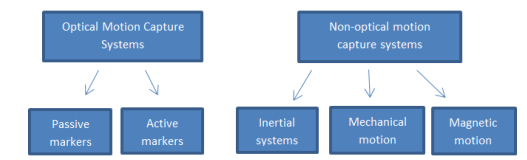
\includegraphics[width=0.7\textwidth]{figures/Mocap.png}
	\caption{MoCap systems Hierarchy}
\end{figure}

Motion analysis data collection protocols, measurement precision, and data reduction models have all been developed to meet the needs of their respective settings. Sport assessments, for example, necessitate higher data acquisition rates due to higher velocities than normal walking. Furthermore, real-time tracking is required for a realistic user experience, so time lag should be kept to a minimum. Years of technological advancement have resulted in numerous systems that can be classified as optical and non-optical, where non-optical category contains mechanical, magnetic, or inertial trackers. The human body is frequently viewed as a network of rigid links connected by joints. Human body parts are not rigid structures, but they are commonly treated as such during human motion studies. 
\subsubsection{Optical Motion Capture}

\begin{figure}[h]
	\centering
	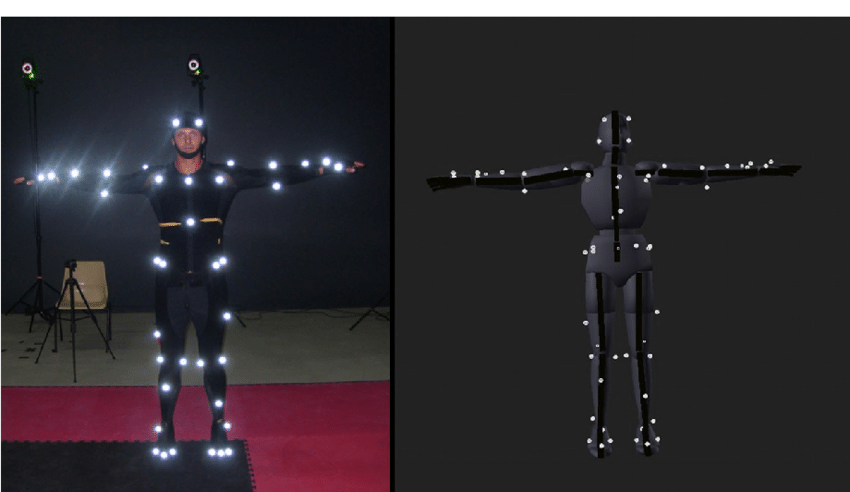
\includegraphics[width=0.6\textwidth]{figures/background/Optical.png}
	\caption{\href{https://www.researchgate.net/profile/Jacek-Hordyj/publication/283152771/figure/fig1/AS:669997391159296@1536751234023/Actor-wearing-suit-adjusted-for-optical-motion-capture-on-the-left-Virtual-model.png}
	{Optical Motion Capture suit}}
\end{figure}

Multiple high-speed cameras   \cite{Optical Motion Capture: Theory and Implementation,MOTION CAPTURE TO BUILD A FOUNDATION FOR A COMPUTER-CONTROLLED INSTRUMENT BY STUDY OF CLASSICAL GUITAR PERFORMANCE} or video cameras are used in optical motion capture systems to triangulate the position of each marker on the actor. This method involves using a series of synchronized cameras to capture markers placed in strategic locations on the body. More specifically, a number of synchronized cameras, an image acquisition system, a capturing area, and a special suit with markers are all required for the implementation of an optical motion capture system.The positions of the markers on the suit are designed to cover the necessary body parts.\\

Passive optical marker systems employ a variety of highly reflective markers of varying sizes that reflect light back to cameras. These markers can be velcroed to a body suit or applied directly to the skin. A ring of visible red, near red, or infrared strobe light emitting diodes (LEDs) around the camera lens generates the reflected light. The cameras' light sensitivity can be adjusted to reject other sources of light. Passive markers have the advantage of not requiring a power source such as batteries, wiring, or other electronic devices. The downside is that to the cameras, all of the markings appear to be the same. This means that if many markers are occluded and subsequently reappear in camera view, the cameras are unable to distinguish between them.\\

Active optical marker systems employ powered LEDs as markers.
Unlike passive markers, which reflect light back to cameras, these markers emit their own visible red or infrared light. These markers, like passive markers, can be adhered directly to the skin or velcroed to a body suit. The advantages of active markers are that each LED modulates and emits a unique frequency, resulting in each marker being uniquely identified. The disadvantage is that each LED must be powered, which necessitates the use of wires and related devices like batteries and circuit boards.
 
\subsubsection{Non-Optical Motion Capture}
\subsubsection*{Inertial Motion Capture}
\begin{figure}[h]
	\centering
	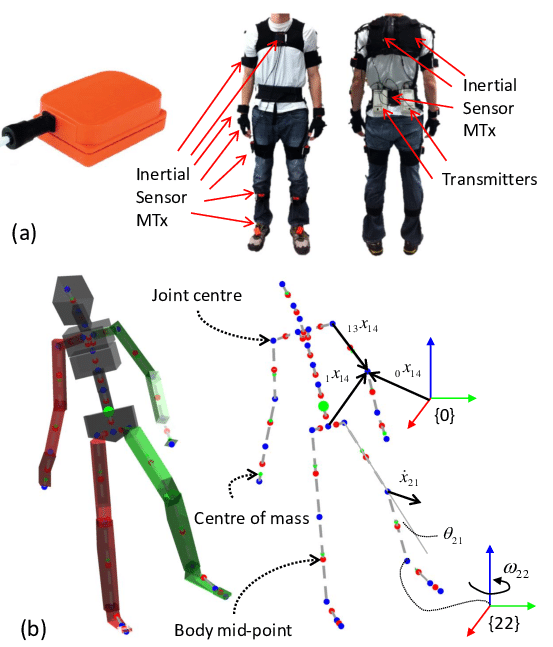
\includegraphics[width=0.4\textwidth]{figures/background/Inertial.png}
	\caption{\href{https://www.researchgate.net/profile/Matthew-Field-6/publication/257308000/figure/fig1/AS:613448983531582@1523269043700/a-The-inertial-sensor-MTx-left-14-and-positioning-of-the-sensors-and-wireless.png}
	{Inertial sensor suit}}
\end{figure}

Inertial sensors \cite{Kalman Filtering for Sensor Fusionin a Human Tracking System} rely on the property of bodies to maintain constant translational and rotational velocity unless perturbed by forces or torques. The vestibular system is a biological 3D inertial sensor located in the inner ear. It can detect both angular motion and linear acceleration of the head. The vestibular system is critical for maintaining eye balance and stabilization in relation to the environment. Advances in miniaturized and micro-machined sensor technologies, particularly silicon accelerometers and rate sensors, have made practical inertial tracking possible. A rate gyroscope measures angular velocity and provides the change in angle with respect to an initially known angle when integrated over time. Accelerations, including gravitational acceleration g, are measured by an accelerometer.\\

If the sensor's angle with respect to the vertical is known, the gravity component can be removed and velocity and position can be calculated using numerical integration. If no compensation is used, the noise and bias errors associated with small and inexpensive sensors make tracking orientation and position for long periods of time impractical. Drift and other errors can be reduced by combining signals from inertial sensors with those from aiding/complementary sensors and using knowledge about their signal characteristics.

\subsubsection*{Mechanical Motion Capture}

\begin{figure}[h]
	\centering
	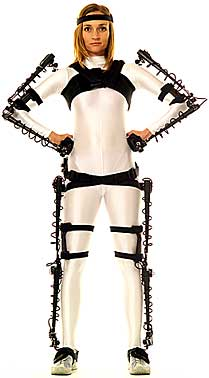
\includegraphics[width=0.3\textwidth]{figures/background/Mechanical.png}
	\captionsetup{labelformat=empty}
	\caption{\href{https://metamotion.com/images/gypsy4_standing.jpg}
	{Mechanical mocap suit}}
\end{figure}

Because of the external structure \cite{MOTION CAPTURE TO BUILD A FOUNDATION FOR A COMPUTER-CONTROLLED INSTRUMENT BY STUDY OF CLASSICAL GUITAR PERFORMANCE} that is attached to the performer, mechanical motion capture systems are also known as exoskeleton motion capture systems. These structures, which are typically made of rigid metal or plastic, have articulated joints with potentiometers that directly measure a performer's joint angles as he or she moves. One of the primary benefits of this direct measurement system is the absence of the need for cameras or other sensors. The system's main drawbacks are that the performer is restricted to the degrees of freedom of the structure and that the location of the sensor placement is fixed. If the performer attempts to move beyond the system's degrees of freedom, the structure may be damaged or broken.

\pagebreak

\subsubsection*{Magnetic Motion Capture}

\begin{figure}[h]
	\centering
	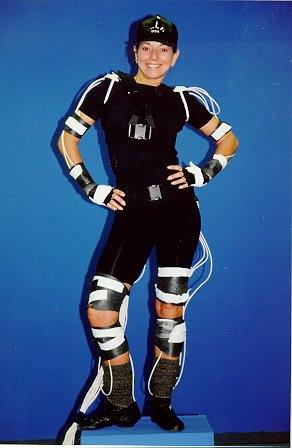
\includegraphics[width=0.3\textwidth]{figures/background/Magnetic.png}
	\captionsetup{labelformat=empty}
	\caption{\href{https://www.researchgate.net/profile/Jessica-Hodgins-2/publication/2359279/figure/fig4/AS:669524957331457@1536638597171/A-performer-wearing-a-motion-capture-apparatus-The-device-shown-is-a-full-body-magnetic.ppm}
	{Magnetic mocap suit}}
\end{figure}

Magnetic motion capture systems \cite{MOTION CAPTURE TO BUILD A FOUNDATION FOR A COMPUTER-CONTROLLED INSTRUMENT BY STUDY OF CLASSICAL GUITAR PERFORMANCE} work by measuring the low-frequency magnetic field produced by a source transmitter and relaying it to a receiver. Each transmitter and receiver have three orthogonal coils that measure magnetic flux between them and calculate the position and orientation of each sensor. One of the key advantages of these systems is that instead of the more conventional three degrees of position, each sensor transmitter/receiver pair may capture both orientation and position. However, sensors in the system, are susceptible to environmental metal, magnetic fields, and electrical sources such as rebar walls and floors, lights, cables, monitors, and computers. Shielding equipment and wiring requires special care. Despite their high accuracy, the sensors become nonlinear at the extremes of their range. 
\subsection{Neural Networks}
\subsubsection{Artificial Neural Network}
Machine Learning methods, particularly Artificial Neural Networks (ANNs), have shown promising capabilities in solving a wide range of complex problems. Neural networks are a class of machine learning techniques that attempts to recognize underlying relationships in a set of data using a process similar to how the human brain works. An artificial neural network (ANN) is a machine learning algorithm inspired by biological neural networks. The nodes in each ANN communicate with one another via connections. A deep network can represent functions of increasing complexity by adding more layers and units within a layer.

\pagebreak

 \begin{figure}[h]
	\centering
	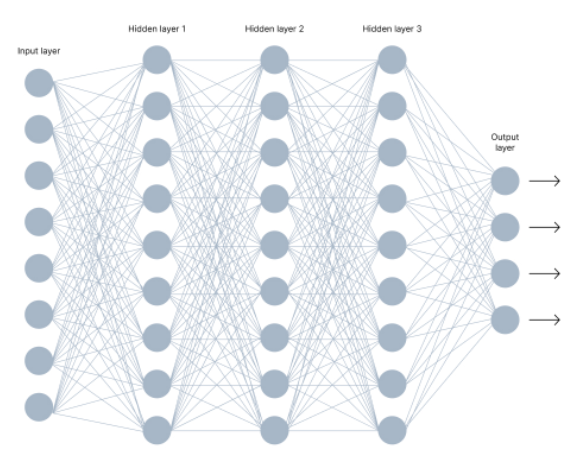
\includegraphics[width=0.6\textwidth]{figures/background/ANN.png}
	\captionsetup{labelformat=empty}
	\caption{\href{https://assets-global.website-files.com/5d7b77b063a9066d83e1209c/60d242974bcba9f8c670e03e_Group\%20806.jpg}
	{Neural Networks Architecture}}
\end{figure}

\subsubsection*{Artificial Neuron}
The fundamental building block of a neural network is a single neuron, which is also
 called a perceptron. More specifically, each neuron is a machine learning method that takes a set of features and their targets as input and tries to discover a line, plane, or hyperplane in two, three, or hyper-dimensional space that separates the classes. The sigmoid function is used to alter these characteristics.
 
 \begin{figure}[h]
	\centering
	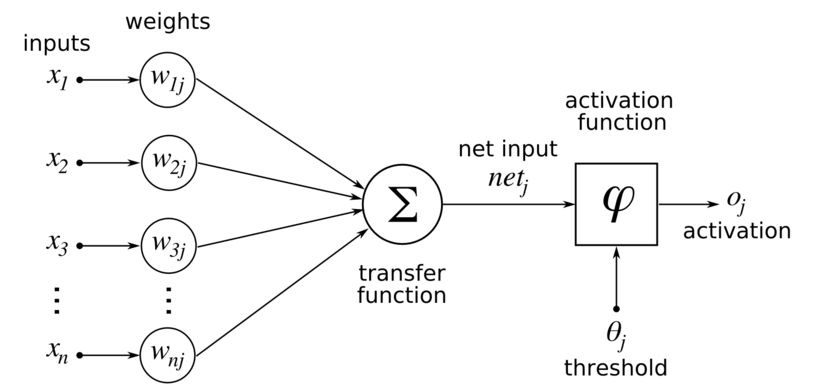
\includegraphics[width=0.6\textwidth]{figures/background/Neuron.png}
	\captionsetup{labelformat=empty}
	\caption{\href{https://commons.wikimedia.org/wiki/File:ArtificialNeuronModel_english.png}
	{Artificial Neuron}}
\end{figure}

Simple ANNs have an input layer and an output layer with zero to three hidden layers, whereas deep neural networks have no limit in the number of hidden layers. Multiple neurons make up a layer of a multilayer perceptron, and the input values as well as the bias values are assigned
during the training process.



\subsubsection*{Activation function}
The Activation function is used to determine whether or not the neuron will be activated. This means that it will use simpler mathematical operations to determine whether the neuron's input to the network is essential or not throughout the prediction phase. These mathematical functions are added to an artificial neural network to assist it in learning complex patterns in data. The reason that activation functions are essential parts of a ANN is that the combination of nonlinear activation functions from different neurons permits the network to approximate complex functions or distributions of data. Simpler, the most important feature of an activation function is to add non-linearity to a neural network. There are many activation functions, but here we show the most used functions.

 \begin{figure}[h]
	\centering
	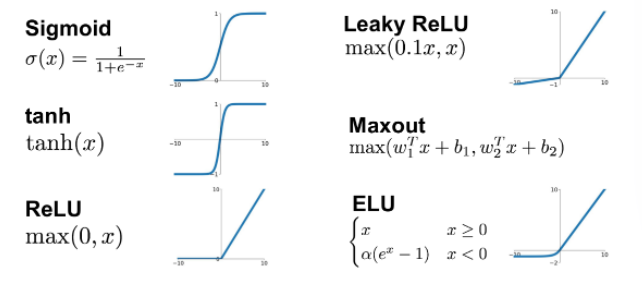
\includegraphics[width=0.6\textwidth]{figures/background/ActivationFunctions.png}
	\captionsetup{labelformat=empty}
	\caption{\href{https://datasciencepreparation.com/blog/articles/what-is-an-activation-function-what-are-commonly-used-activation-functions/}
	{Most common activation functions}}
\end{figure}

\subsubsection*{Loss Function}

One of the most important aspects of an ANN is the choice of the loss function \cite{The importance of the loss function in option valuation} . A loss function is incredibly simple at its core: It's a technique for determining how well your algorithm models your dataset. If the ANN predictions are completely incorrect, the loss function will return a higher value. Otherwise, it will return a lower value. However, minimizing the loss function doesn't necessarily mean that the prediction is getting closer to the desired results. There are some well-known categories of loss functions that may work on many simple ANN, but if the problem that the ANN has to solve is too complicated, it may need a custom loss function, that is special for the specific problem and ANN architecture. \\

In particular, the purpose of a loss function in an ANN is to adjust the weights and the bias during the training. If we could, we would find the perfect weights and bias for our ANN, but it has not yet been proven a formula that could do it. Therefore, these functions will try to find the adjustments, that are as close as to the perfect one's. \\

Pressingly, the loss function that is used is directly related to the activation function that is used in the neural network's output layer. Consider the output layer configuration to be a choice about the framing of the prediction problem, and the loss function selection to be the method for calculating the error for a given framing of the problem. The loss functions can be classified into two major categories depending upon the type of learning task we are dealing with Regression losses and Classification losses. In classification, we are trying to predict output from set of finite categorical values. Regression, on the other hand, deals with predicting a continuous value.

\subsubsection*{Back-propagation}

 \begin{figure}[h]
	\centering
	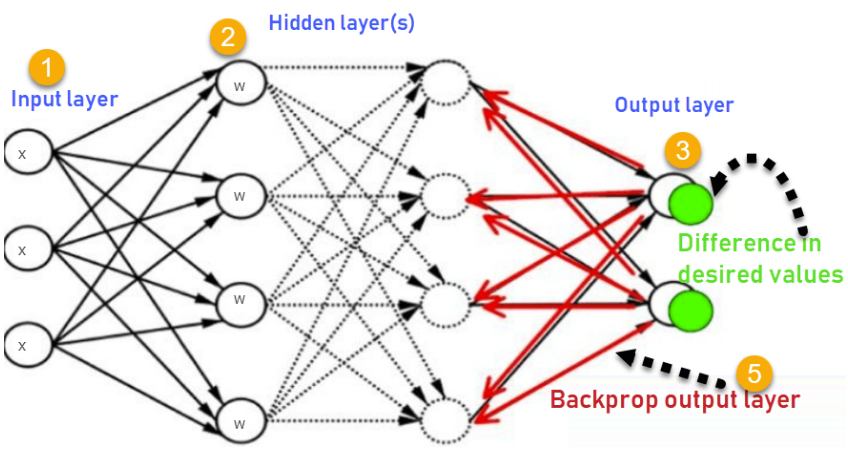
\includegraphics[width=0.8\textwidth]{figures/background/Backpropagation.png}
	\captionsetup{labelformat=empty}
	\caption{\href{https://www.guru99.com/images/1/030819_0937_BackPropaga1.png}
	{Backpropagation Algorithm}}
\end{figure}


The essence of neural net training is back-propagation. It is the practice of fine-tuning a neural net's weights based on the error rate obtained in the previous epoch. Proper weight tuning ensures lower error rates, increasing the model's reliability by increasing its generalization. \\

The back-propagation algorithm in neural networks computes the gradient of the loss function for a single weight using the chain rule. Unlike native direct computation, it efficiently computes one layer at a time. The back-propagation algorithm, allows the information from the cost to then flow backwards through the network, in order to compute the gradient. Back-propagation refers only to the method for computing the gradient, while another algorithm,
such as stochastic gradient descent, is used to perform learning using this gradient.

 
\subsubsection{Convolutional Neural Network}
Convolutional networks, \cite{Deep Learning} also known as convolutional neural networks or CNN, are a specialized kind of artificial neural network for processing data that has a known, grid-like topology. Examples include time-series data, which can be thought of as a 1D grid taking samples at regular time intervals, and image data, which can be thought of as a 2D grid of pixels. Convolutional networks are simply neural networks that use convolution in place of general matrix multiplication in at least one of their layers.\\

The main strengths of CNNs are to provide an efficient dense network which performs the prediction or identification etc. efficiently. CNNs are the most popular topic in the pool of deep learning, which is indeed very vast, and this is usually because of the ConvNets. Immense datasets are applied to CNNs, it is even considered that larger the data, greater the accuracy will result, otherwise other operations such as transfer learning shall be applied to expand the data. The power of CNN is to detect distinct features from images all by itself, without any actual human intervention.\\

There are multiple benefits of using this model as the state of art neural network. As it can be used in various fields and perform major tasks like facial recognition, analyzing documents, understanding climate, and image recognition and object identification etc. Deep learning has helped enormously in advancement of the science fields and CNN is the most popular one as it attains the benefits of providing maximum performance and efficiency.\\

Traditional neural network layers use matrix multiplication by a matrix of
parameters with a separate parameter describing the interaction between each input
unit and each output unit. This means every output unit interacts with every input
unit. Convolutional networks, however, typically have sparse interactions (also
referred to as sparse connectivity or sparse weights). This is accomplished by
making the kernel smaller than the input. For example, when processing an image,
the input image might have thousands or millions of pixels, but we can detect small,
meaningful features such as edges with kernels that occupy only tens or hundreds of
pixels. This means that we need to store fewer parameters, which both reduces the
memory requirements of the model and improves its statistical efficiency. It also
means that computing the output requires fewer operations. These improvements
in efficiency are usually quite large. If there are m inputs and n outputs, then
matrix multiplication requires m x n parameters and the algorithms used in practice
have O(m x n) run-time. If we limit the number of connections
each output may have to k, then the sparsely connected approach requires only
k x n parameters and O(k x n) run-time. For many practical applications, it is
possible to obtain good performance on the machine learning task while keeping
k several orders of magnitude smaller than m. \\


Each convolutional layer contains a series of filters known as convolutional kernels. The filter is a matrix of integers that are used on a subset of the input pixel values, the same size as the kernel. Each pixel is multiplied by the corresponding value in the kernel, then the result is summed up for a single value for simplicity representing a grid cell, like a pixel, in the output channel/feature map. In computer vision the input is often a 3 channel RGB image. For simplicity, if we take a grey-scale image that has one channel (a two dimensional matrix) and a 3x3 convolutional kernel (a two dimensional matrix). The kernel strides over the input matrix of numbers moving horizontally column by column, sliding/scanning over the first rows in the matrix containing the images pixel values. Then the kernel strides down vertically to subsequent rows. Note, the filter may stride over one or several pixels at a time, this is detailed further below.


 \begin{figure}[h]
	\centering
	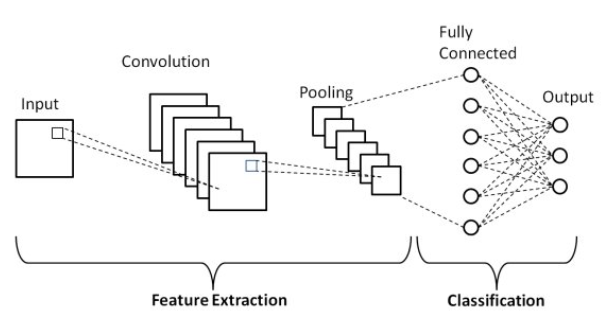
\includegraphics[width=0.8\textwidth]{figures/background/CNN.png}
	\captionsetup{labelformat=empty}
	\caption{\href{https://www.researchgate.net/publication/336805909/figure/fig1/AS:817888827023360@1572011300751/Schematic-diagram-of-a-basic-convolutional-neural-network-CNN-architecture-26.ppm}
	{Basic Convolution Neural Network Architecture}}
\end{figure}

\subsection{Related Work}
Recent work in the computer graphics and vision sectors have focused on developing digital tools for reconstructing, tracking, and evaluating human motion using visual input. More specifically, these digital tools that are easier and much cheaper to use, than mocap suits, and in the near future these methods have the potential to surpass the current technology that we talked about in the previous sections. At the moment, the resulting quality of these tools is not as good as the current technology, but many scientists propose state-of-the-art approaches in order to improve them.\\  

 \begin{figure}[h]
	\centering
	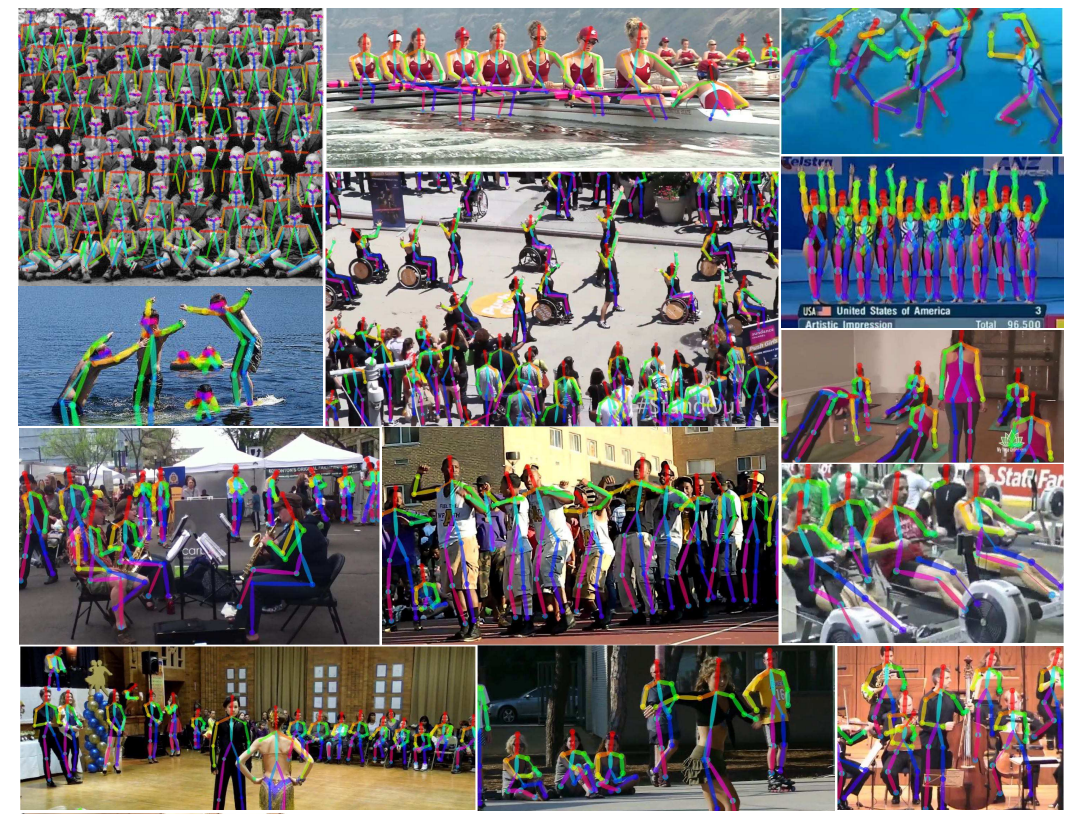
\includegraphics[width=0.6\textwidth]{figures/background/2D.png}
	\caption{\href{https://openaccess.thecvf.com/content_cvpr_2017/papers/Cao_Realtime_Multi-Person_2D_CVPR_2017_paper.pdf}
	{2D Multi-Person high accuracy human Pose estimation}}
\end{figure}

Reconstructing 3D human poses from real-world images in a variety of indoor and outdoor scenarios has a wide range of applications in entertainment, environmental awareness, and human-computer interaction. There are some ways to achieve that, but we will focus more on a specific procedure that estimates 3D human poses from a list of images or a video. Firstly, we will extract the 2D human poses from each image using some well-known Neural Networks specifically trained for this job. In particular, deep neural networks \cite{OpenPose,HrNet,AlphaPose} have revolutionized  2D pose estimation, producing accurate predictions even for poses with self-occlusions. These Neural Network can estimate the 2D human Pose in Real-Time with  high accuracy. These networks were trained with COCO dataset,  which contains over 200, 000 images and 250, 000 person instances labeled with 17 keypoints that are very easily recognisable. Even though the main difference in these network is the architecture and the training the 2D human Pose estimation, is very close. The main difference is the speed of the model and the hardware requirements of each model.\\

\pagebreak

 \begin{figure}[h]
	\centering
	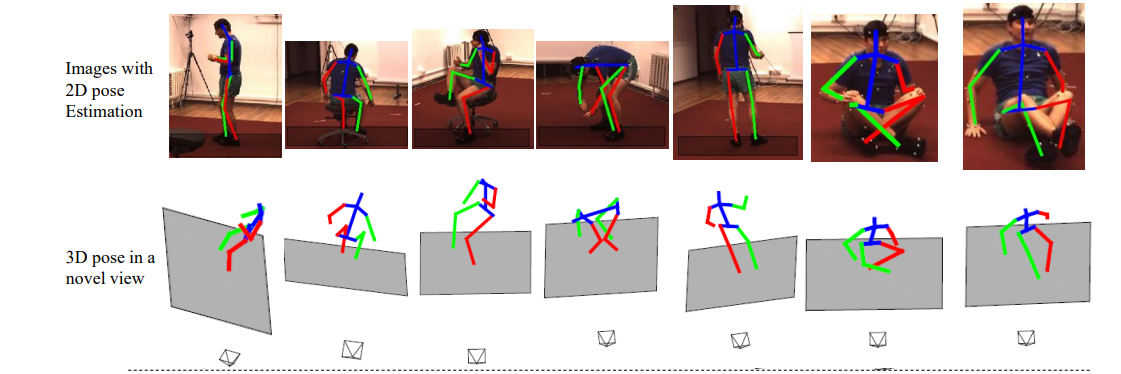
\includegraphics[width=1\textwidth]{figures/background/2D&3D.png}
	\caption{\href{https://arxiv.org/pdf/1612.06524.pdf}
	{2D and 3D human Pose difference in estimation}}
\end{figure}

In the last decade, the research community has paid close attention to inferring the 3D human pose from images or video. All the following studies \cite{Exploiting temporal information for 3D pose estimation,3D Human Pose Estimation from Deep Multi-View 2D Pose,3D Human Pose Estimation Using Convolutional Neural Networks with 2D Pose Information,3D Human Pose Estimation = 2D Pose Estimation + Matching}are proposing a deep neural network that can estimate 3D human poses  from a sequence of 2D human poses. Even though that each paper, proposes a different neural network architecture, all of them uses Human3.6M dataset and some of them, add to the training some other smaller datasets for further improvement of the results.\\

 \begin{figure}[h]
	\centering
	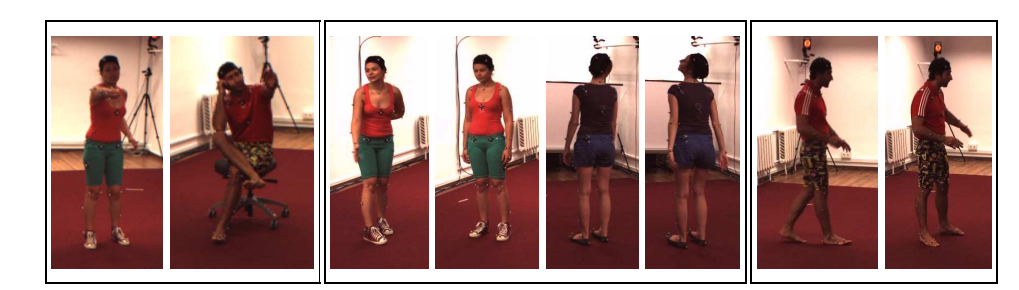
\includegraphics[width=1\textwidth]{figures/background/human36M.png}
	\caption{\href{https://vision.imar.ro/human3.6m/pami-h36m.pdf}
	{Examples of human poses in the Human3.6M dataset}}
\end{figure}

Recently, there has been some interest in systems whose components are trained using datasets of human motion capture . More specifically, a well-known and most used dataset is Human3.6M \cite{Human3.6M} which is a dataset of 3.6 million accurate 3D human poses collected by recording the performance of 5 female and 6 male subjects from four different perspectives in order to train realistic human sensing systems and evaluate the next generation of human pose estimation models and algorithms. \\



 
\subsection{Gait mocap clip Generation through a GAN}
All these methods try to estimate the 3D human Pose from a video. Another very interesting approach is to try to generate a BVH file that contains the mocap human pose information. The neural network that can achieve such task is a Generative adversarial network (GAN) \cite{ANIMGAN}. A GAN contains two neural networks the discriminator and the generator. Before the training starts, the former learns to separate fake data from real, and in the case of a fake, it includes how far it is from being real. The latter is creating some data, and its goal is to fool the discriminator by creating virtual data that looks real. Moreover in GAN's many researchers uses a type of layer, Long Short-Term Memory (LSTM) that are a type of recurrent neural network capable of learning order dependence in sequence prediction problems. Simply, this layer tries to find every association of the data, in our case, the association between the neighbours frames of the video. So, this paper, proposed a spatiotemporally-conditioned
GAN that generates a sequence that is similar to a given sequence in terms of semantics and spatiotemporal dynamics.Using LSTM-based generator and graph ConvNet discriminator, this system is trained end-to-end on a large gathered dataset of gestures, expressions, and actions.
\subsubsection{Data Augmentation}
There are not many different walking datasets that can be used for this work. More specifically, Carnegie Mellon University which was created a huge motion capture dataset a decade ago that will be used in this Thesis. Moreover, It is possible for the skeleton that CMU proposed, to be rigged to a mixamo or another more modern skeleton through the blender and eventually import to game engines like Unity. This also means that we can increase the quantity of the CMU dataset by adding some mixamo or other well-known motion capture datasets (in BVH format) clips.\\

The CMU Graphics Lab Motion Capture Database (CMU) is by far the most extensive dataset of publicly available motion capture data. Many researchers within the community have used it to build prior models of human motion. This dataset was in Acclaim format. In particular, the Acclaim format is made up of two files, a skeleton file and a motion file. This was done knowing that a single skeleton works for many different motions most of the time and rather than storing the same skeleton in each of the motion files, it should be stored just once in another file. The skeleton file is the ASF file (Acclaim Skeleton File). The motion file is the AMC file (Acclaim Motion Capture data). In addition, some people created python software that converts the Acclaim files into BVH files. It means that these files can be imported into the blender for further usage.\\

There some other datasets like mixamo, that contains high-quality motion capture but it is not always free. The primary purpose of these motion capture is game construction of video clip animation. In this thesis, it is important to obtain a significant amount of motion capture, something that only CMU can offer for free. Fortunately, we can still modify the mixamo dataset (rig the mixamo skeleton to CMU skeleton) and merge it to the CMU dataset.\\

This dataset will train a neural network to classify for the training when the skeleton model
of the dataset is walking. Some approaches train a neural network with the CMU mocap
clips as the dataset. The CMU skeleton has 31 joints, and each joint is described by the
position (XYZ) and the rotation (XYZ), a total of 6 variables. That sum up to 186 variables
for each frame. Each clip has 3198 frames, and we use 1073 clips from the dataset. So the
dataset final form is a array with  these dimensions (1073,3198,186).\\

In addition to these clips, we added some noise z using a normal or uniform distribution to some of the clips in order to classify some of them as fake. This was necessary for the network, in order to understand, during the training what a  false sample looks like. So, the now has a form of (1500,3198,186), which means that we were added 427 false samples. \\

However, it is still a small dataset. There a machine learning strategy, that allows you to increase your dataset, it is called data augmentation. More specifically, data augmentation is a strategy that enables practitioners to significantly increase the diversity of data available for training models, without actually collecting new data. The data augmentation in our case includes random rotation ([-$45^o$, $45^o$]) and random scale ([0.5, 1.5]). So the final form of the dataset was (10000,3198,186).
\subsubsection{Dataset}
There are not many different walking datasets that can be used for this work. More specifically, Carnegie Mellon University which was created a huge motion capture dataset a decade ago that will be used in this Thesis. Moreover, It is possible for the skeleton that CMU proposed, to be rigged to a mixamo or another more modern skeleton through the blender and eventually import to game engines like Unity. This also means that we can increase the quantity of the CMU dataset by adding some mixamo or other well-known motion capture datasets (in BVH format) clips.\\

The CMU Graphics Lab Motion Capture Database (CMU) is by far the most extensive dataset of publicly available motion capture data. Many researchers within the community have used it to build prior models of human motion. This dataset was in Acclaim format. In particular, the Acclaim format is made up of two files, a skeleton file and a motion file. This was done knowing that a single skeleton works for many different motions most of the time and rather than storing the same skeleton in each of the motion files, it should be stored just once in another file. The skeleton file is the ASF file (Acclaim Skeleton File). The motion file is the AMC file (Acclaim Motion Capture data). In addition, some people created python software that converts the Acclaim files into BVH files. It means that these files can be imported into the blender for further usage.\\

There some other datasets like mixamo, that contains high-quality motion capture but it is not always free. The primary purpose of these motion capture is game construction of video clip animation. In this thesis, it is important to obtain a significant amount of motion capture, something that only CMU can offer for free. Fortunately, we can still modify the mixamo dataset (rig the mixamo skeleton to CMU skeleton) and merge it to the CMU dataset.\\

This dataset will train a neural network to classify for the training when the skeleton model
of the dataset is walking. Some approaches train a neural network with the CMU mocap
clips as the dataset. The CMU skeleton has 31 joints, and each joint is described by the
position (XYZ) and the rotation (XYZ), a total of 6 variables. That sum up to 186 variables
for each frame. Each clip has 3198 frames, and we use 1073 clips from the dataset. So the
dataset final form is a array with  these dimensions (1073,3198,186).\\

In addition to these clips, we added some noise z using a normal or uniform distribution to some of the clips in order to classify some of them as fake. This was necessary for the network, in order to understand, during the training what a  false sample looks like. So, the now has a form of (1500,3198,186), which means that we were added 427 false samples. \\

However, it is still a small dataset. There a machine learning strategy, that allows you to increase your dataset, it is called data augmentation. More specifically, data augmentation is a strategy that enables practitioners to significantly increase the diversity of data available for training models, without actually collecting new data. The data augmentation in our case includes random rotation ([-$45^o$, $45^o$]) and random scale ([0.5, 1.5]). So the final form of the dataset was (10000,3198,186).
\subsubsection{Generative Adversarial Networks}
Unfortunately, the results of this approach were terrible. The main reason was the small dataset that we were able to find for free. Even though we tried to do data augmentation in our dataset, there is a limitation. The main limitation of data augmentation arises from the data bias, i.e. the augmented data distribution can be quite different from the original one. This data bias leads to a sub-optimal performance of existing data augmentation methods. In particular, the generator could not improve his results, so the output was something a little better than the  noise z using a normal or uniform distribution that we sampled in the generator in the initial phase and the humanoid was doing independent random moves in each frame of the motion. The dataset limitation in this area is something that many researchers have noticed, and the goal was to try to increase the dataset even with poorer quality with this model. 
\subsubsection{Evaluation of the approach}
Unfortunately, the results of this approach were terrible. The main reason was the small dataset that we were able to find for free. Even though we tried to do data augmentation in our dataset, there is a limitation. The main limitation of data augmentation arises from the data bias, i.e. the augmented data distribution can be quite different from the original one. This data bias leads to a sub-optimal performance of existing data augmentation methods. In particular, the generator could not improve his results, so the output was something a little better than the  noise z using a normal or uniform distribution that we sampled in the generator in the initial phase and the humanoid was doing independent random moves in each frame of the motion. The dataset limitation in this area is something that many researchers have noticed, and the goal was to try to increase the dataset even with poorer quality with this model. 

\newpage
\section*{Chapter 3 \\}
\section{Requirements}
\subsection{Hardware}
As we mentioned in previous sections, models that estimate human pose, particularly models that estimate 2D poses from a single image, require above-average hardware. These models can be loaded on the CPU but the speed that the model needs to run the estimation is about 0.2-0.3 frames per second in Intel Core i7-7700HQ (2.8GHz) which is considered an above-average CPU. On the other hand, having a GPU with at least 2 GB VRAM (that is the minimum allocated space that the models need to be loaded), the speed that the model needs to run the estimation is about 4-5 frames per second in NIVIDIA GeForce GTX 1050 which also is considered an above-average GPU. The difference in speed is enormous, GPU is about 20 times faster than the CPU. The application was tested on a laptop, MSI GL72M 7RDX. During the run-time, the hardware of the laptop is shown in the figure from the application MSI DRAGON CENTER:

\begin{figure}[h]
	\centering
	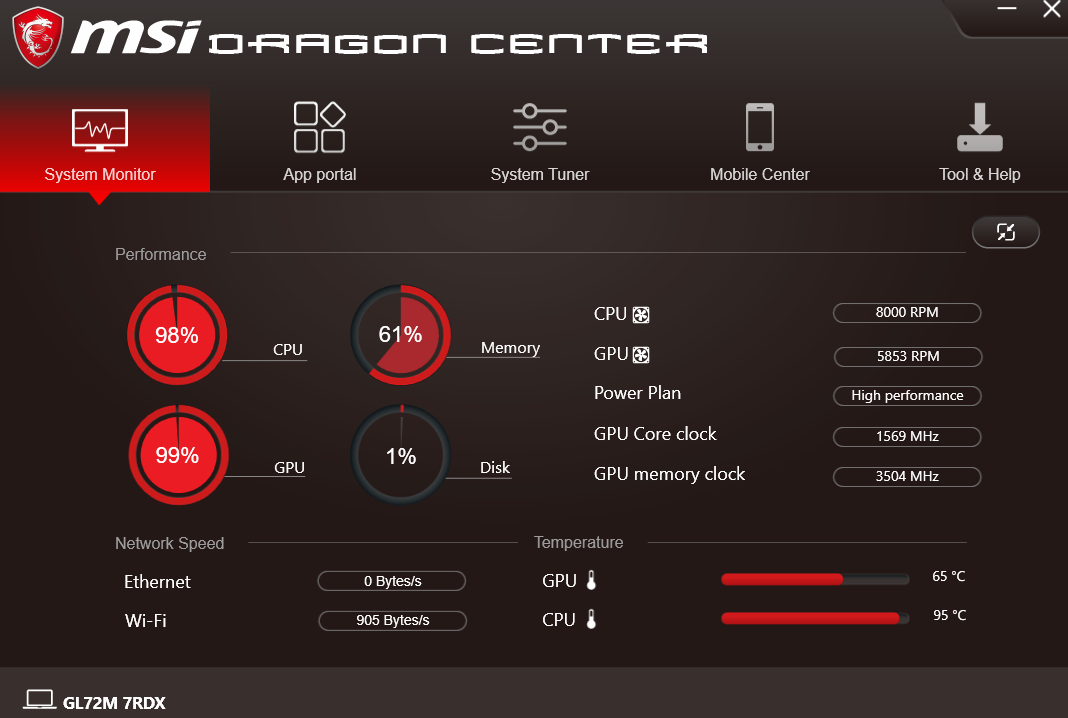
\includegraphics[width=0.9\textwidth]{figures/Requirements/Perfomance.png}
	\captionsetup{labelformat=empty}
	\caption{ MSI GL72M 7RDX performance stats}
\end{figure}
\subsection{Input requirements}
The input of the algorithm is a video. We suggest that the resolution of the video is at least 720p, in order that every human joint can be easily recognizable by the model. The best video resolution for the specific version of the application is 1080p, which maximizes the algorithm speed as well as the resulting quality. However, the results (depends on the movement complexity) may not be clear enough to be imported directly to a game engine studio so this application is addressed to animators. Nevertheless, mocap clips always needed to be cleared (discard some frames and keep the best for the motion), so it was something to be expected. Moreover, there are some rules that if the video-creator follow, he will improve the quality of the model estimation. Firstly, the camera should be motionless, because it affects the position estimation. Secondly, the person's joints should be visible, otherwise, the model may struggle to specify left from right joints, (legs and arms). Another tip is that whole body of the person should be visible for every frame of the video, and the distance between him and the camera should be greater than two meters and less than six meters. The most important idea that would help improve the estimation quality would be if the user could upload a slow-motion video, that will contain the motion of the video in great detail since all the sharp movement will now become smoother, more detailed, and slower between each frame movements.
\pagebreak
\subsection{Application's Workflow}
The Application's workflow can be divided into three parts. The first part is quite simple, the user imports the video of his preference into the Application chooses the folder that he wants to save the results, and presses submit as it is shown in the figures above. 

\pagebreak

\begin{figure}[htp]
	\centering
	{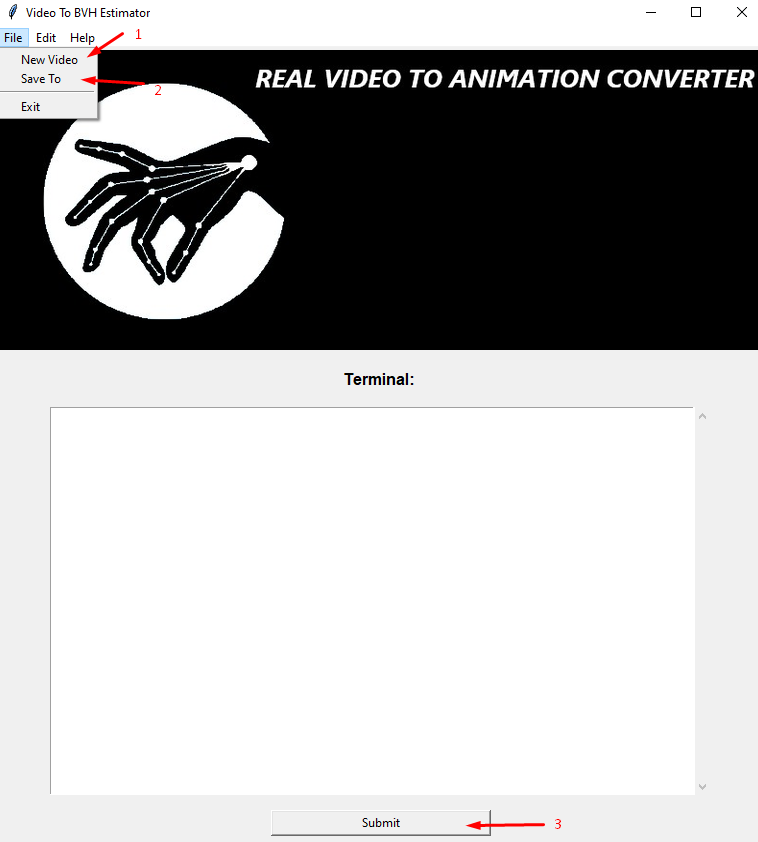
\includegraphics[height=9cm,width=0.48\linewidth]{figures/Requirements/Workflow1_1.png}}
	\hspace{1em}%
	{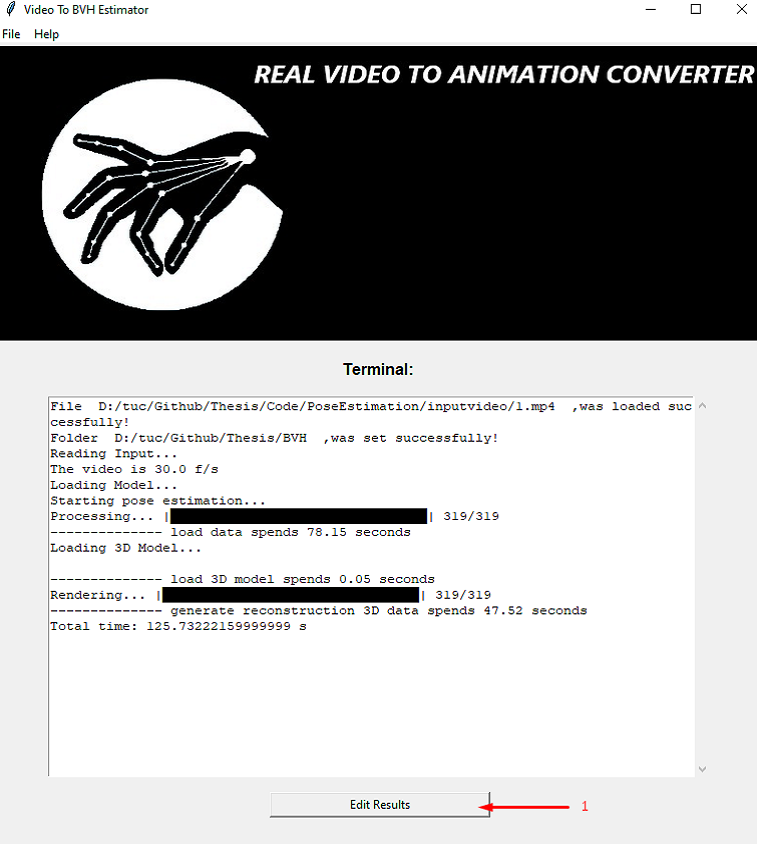
\includegraphics[height=9cm, width=0.48\linewidth]{figures/Requirements/Workflow1_2.png}}
	\captionsetup{labelformat=empty}
	\caption{Input Phase}
\end{figure}

In the above figure, in the left image, we show how to give new input to the Application. In the right image, we show the results that the user should see after a successful video to animation conversion as well as the way to go to the next panel.\\\\


 \begin{figure}[h]
	\centering
	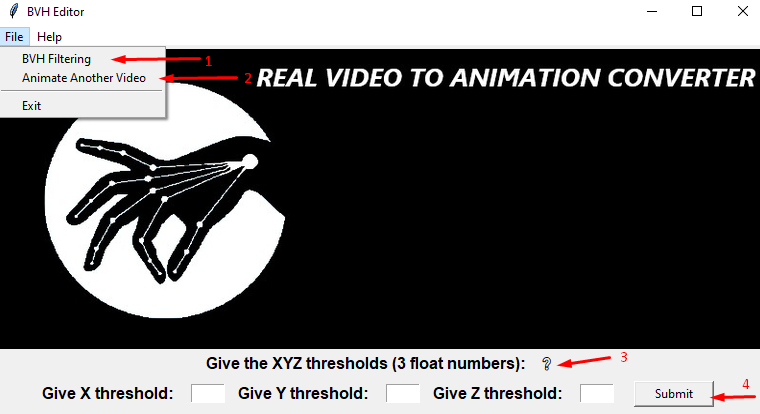
\includegraphics[width=0.55\textwidth]{figures/Requirements/Workflow2_1.png}
	\captionsetup{labelformat=empty}
	\caption{Editing Phase}
\end{figure}

\pagebreak

In the above figure, in the top image, the user can multiply with a number of his preference for each dimension in $R^3$. By doing so, he can increase or decrease the position speed. In the right image, the user can press the left button to filter the BVH motion data in order to reduce the noise, or can press the right button in order to return to the first panel and animate more videos. In addition, if the user does not understand something from the application, he can hover the mouse over the question marks to display some tips.\\\\


\begin{figure}[htp]
	\centering
	{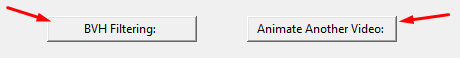
\includegraphics[height=10cm,width=0.48\linewidth]{figures/Requirements/Workflow2_2.png}}
	\hspace{1em}%
	{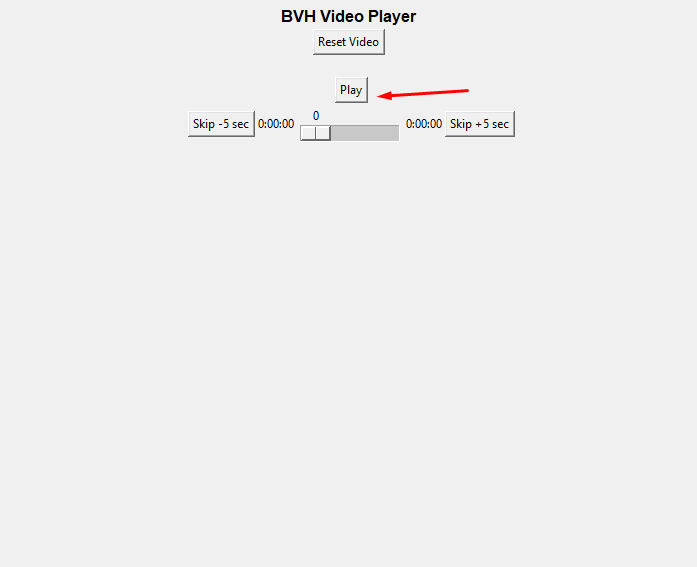
\includegraphics[height=10cm, width=0.48\linewidth]{figures/Requirements/Workflow2_3.png}}
	\captionsetup{labelformat=empty}
	\caption{BVH Video Player}
\end{figure}

The animators may change several things during this phase, so it would be very helpful if they could actually see the motion displayed in this panel. Therefore, if the pressed play, an mp4 of the motion starts playing. If the user changes something in the motion, either they filter the BVH or edit the position of the skeleton, in order to reload the mp4, they need to press reset the video. Unfortunately, this procedure is time-consuming, depending form the CPU the user has the speed of conversion from a BVH to an mp4, is about 10 frames per second.

\pagebreak

\begin{figure}[htp]
	\centering
	{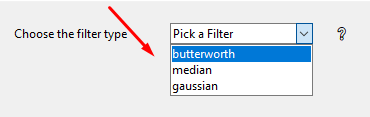
\includegraphics[height=3cm,width=0.48\linewidth]{figures/Requirements/Workflow3_1.png}}
	\hspace{1em}%
	{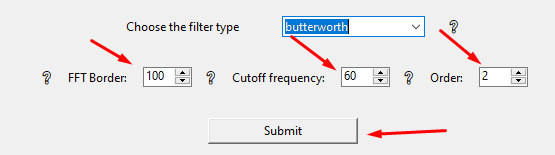
\includegraphics[height=3cm, width=0.48\linewidth]{figures/Requirements/Workflow3_2.png}}
	\captionsetup{labelformat=empty}
	\caption{Filtering Phase}
\end{figure}

In this phase the user can choose a filter of his preference, and insert the parameters that each filter need in order to work. The filter feature is added due to the fact that the estimation that the neural networks do, contain some noise, and these filters can significantly reduce it, or in some cases almost vanished it, which saves a lot of time from the animators.

\newpage
\section*{Chapter 4 \\}
\section{Implementation}
In this thesis, we developed an algorithm based on some well-known pre-trained deep neural networks, that can estimate the 3D human pose from a video. Therefore, we converted these 3D coordinates into a BVH file, that contains a humanoid with 17 bones. In addition, we created a tool that is useful to all the animators who will use our algorithm. This tool can be used to clear the noise of the BVH files with some signal processing filters, to manually fix the location of the humanoid in the space, and to display the results. Finally, we retarget the animation to an avatar that we found online, to show that the animators can use this animation for any other character of their preference. \\

Both the algorithm and the tool were implemented in python. However, this thesis is addressed to animators, and many animators do not have good enough python knowledge to run the code. Therefore, with the help of the Tinker python library, we converter the raw Python Code into a Windows Application that has a very friendly user environment. Even though that with the raw python code, animators can adjust the code to solve their problems, the windows application that we created, in general, can help them solve many things that may need.
\subsection{Benefits of Using Pretrained Models}
As we discussed in the previous sections, the first step that we need to implement in order to estimate the 3D human pose from a video is to estimate the 2D human pose \cite{Exploiting temporal information for 3D pose estimation,3D Human Pose Estimation = 2D Pose Estimation + Matching}. Therefore, we have to find a deep neural network that can do such a task. There are two different ways that we could follow here. \\

On the one hand, we could build a deep neural network from scratch, which is definitely not an easy task to do. This is a very time-consuming procedure since someone must find a promising architecture for the model, and find an enormous Dataset that most of the time needs editing and is not free. However, the training of the deep neural network is the major problem, especially in our case. The goal of the training is to find the ideal parameters that will minimize the loss function of the network. An epoch is one complete pass of the training dataset through the algorithm, and the network has to run many epochs during training to calibrate its weights and bias. Neural network training is a very slow process that depends on the machine that the DNN runs as well as the Dataset size and the training parameters (batch size, early stop, etc.). In our case, the Dataset size that relatives work use contains videos that are many Terabytes of data, which is an enormous amount. Therefore, the training even though a single epoch needs many hours in a state-of-the-art machine learning graphic card, means that in our system would too much time (even days). So, even though we would build our network, the drawbacks are too many, leaving this option as a last resort.\\

On the other hand, we could search to find a pre-trained deep neural network that does our job. Luckily for us, some pre-trained models are trained to estimate exactly what we needed. These models were constructed by many researchers (professors, Ph.D. students, etc.). They had a budget, that helped them find a great Dataset, as well as the latest technology Hardware to train the DNN. The models that we are discussing are  AlphaPose and OpenPose. All of them can estimate the 2D human pose from an image or a sequence of images with great accuracy. These models are trained to do much more than we need in this thesis. They can estimate in Real-time the 2D human pose from a Web-Cam and they can detect and estimate the 2D human pose from multiple people at once. We only need to estimate the pose from a single person from a video. By reading the documentation of these models, we can achieve that.\\

The most important advantage of using a pre-trained model, that satisfies our needs, is that we can avoid all the drawbacks that we discussed in the case that we would create our model. In our case, these models are very powerful, they have great accuracy, so they do not even need further training.
\subsubsection{Available 2D pose estimation Pretrained Models}
As we discussed in the previous section, we decided that we would try to find some available pre-trained models that satisfy our needs. We found 2 models that could use to estimate the 2D human pose from images (AlphaPose and OpenPose). The main difference in these models is the model size, the number of key points that each model predicts per human, and the speed of each model. The accuracy is great for all the models, so it was not a factor to consider. The speed of each model was one of the major factors of each model. Our Hardware could support loading the model on GPU only in the case of the AlphaPose model (which needed 2 GB of VRAM) when the other needed over 3 GB of VRAM. Due to this fact, the difference in speed in AlphaPose was over 30 times faster than the other two models. Another important factor is that AlphaPose had fewer key points, which means that it will have greater accuracy, but poorer quality. At the moment the goal is to create a more stable result, rather than a more attractive one.\\

All the models use the same technique to estimate the 2D pose from the images. They try to estimate some points in the image (x,y) for each joint that they try to find. Therefore, the models predict 18 key points per human that they find in the image, and then with a python library cv2, we connect the dots to create the humanoid. Simpler, having a skeleton with 18 bones, the skeleton from COCO Dataset, the models try to adjust it in every human that they detect in the image. The figures below, demonstrate this procedure.


\begin{figure}[htp]
	\centering
	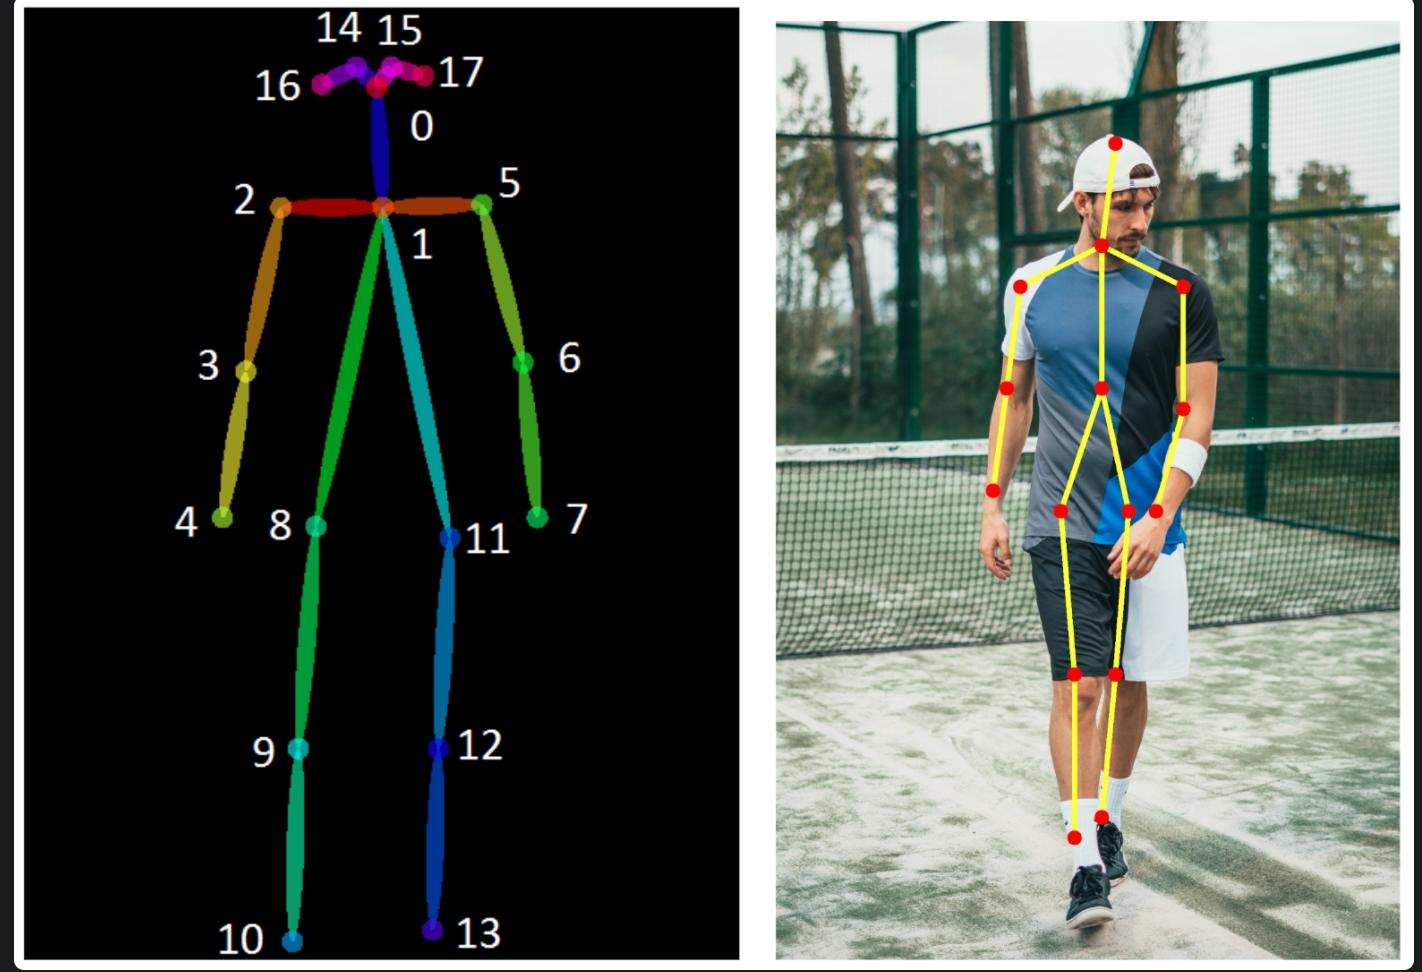
\includegraphics[width=1\textwidth]{figures/Implementation/skeleton.png}
	\captionsetup{labelformat=empty}
    \caption{\href{https://i.stack.imgur.com/sdwNy.jpg}
	{COCO Skeleton that all the models use}}
	\hspace{1em}%
	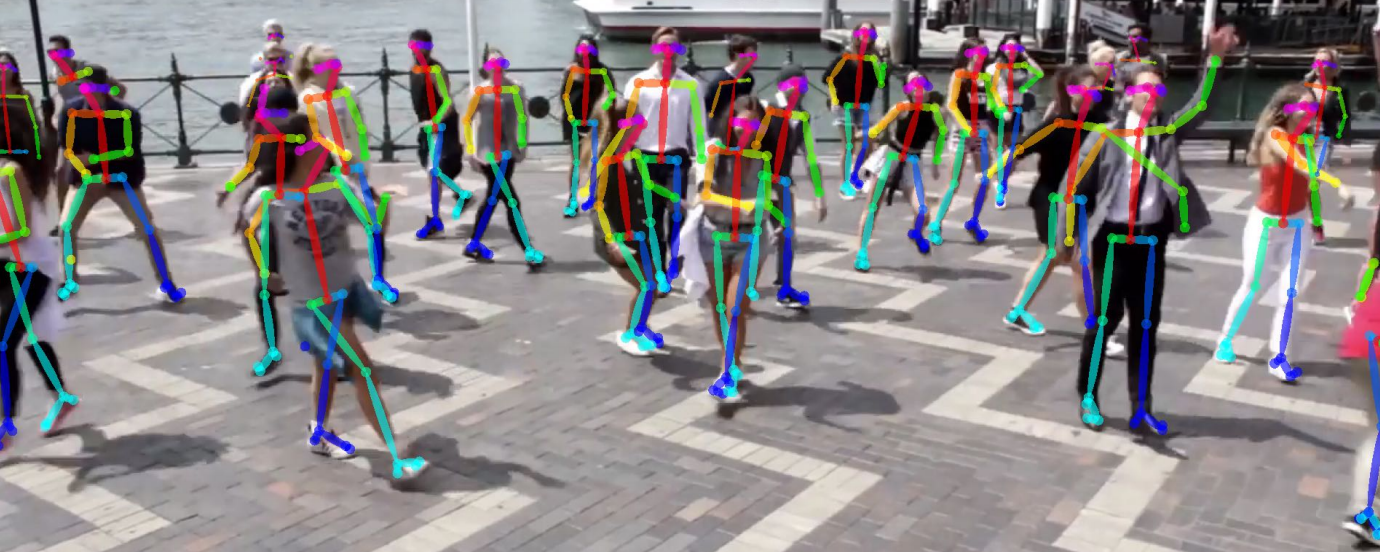
\includegraphics[width=1\textwidth]{figures/Implementation/MultiPerson.png}
	\captionsetup{labelformat=empty}
	\caption{\href{https://github.com/CMU-Perceptual-Computing-Lab/openpose}
	{2D Multi-Human pose Estimation Example}}
\end{figure}

\pagebreak

 \begin{figure}[h]
	\centering
	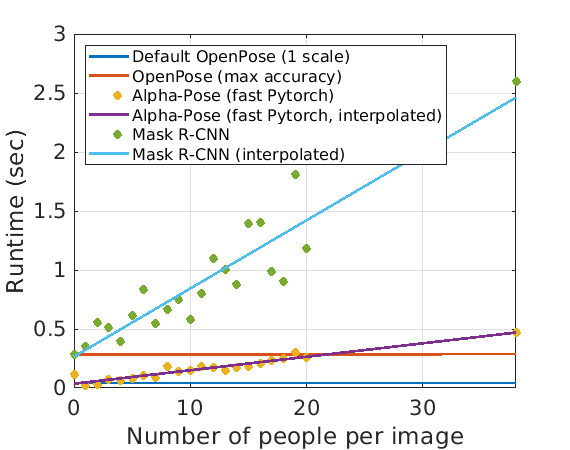
\includegraphics[width=0.75\textwidth]{figures/Implementation/openpose_vs_competition.png}
	\captionsetup{labelformat=empty}
	\caption{\href{https://raw.githubusercontent.com/CMU-Perceptual-Computing-Lab/openpose/master/.github/media/openpose_vs_competition.png}
	{Comparison of each model speed in 2D Multi-Human Pose Estimation}}
\end{figure}

OpenPose model is better and faster when someone wants to detect all the humans that participate in a single image, something that we do not need in this thesis. In the first figure, we show the 2D multi-human pose estimation in an image. In addition, in the second figure, we show the run-time growth for some models with the number of people in the image. Therefore, in our case, for one single person, AlphaPose is the best model in speed and still maintains its max accuracy. Moreover, this OpenPose pre-trained model couldn't be loaded into our GPU, since it wanted more VRAM than we had. Therefore, we would not be able to use this model. In contrast, AlphaPose model could be loaded in our GPU so this played a very important factor when we were choosing the 2D model detector that we were going to use.\\


\subsubsection*{AlphaPose Method}

AlphaPose is a top-down pose estimation algorithm, which chooses Yolo \cite{YOLO-Pose,YOLOv3} as human detector and a single person pose estimator (SPPE) \cite{SPPE} with sequential architecture that detects the human keypoints\\

Yolo model, can classify 80 different objects and segment them inside a box. In our case, the only classification that we need is the human classification, so we can simplify the model in order to get the results faster. Therefore, this model can separate inside a box each human that it can find. Then for each box, we have a single person, and in our case, we will have only one box per frame, since we only accept videos that contain only a single person. \\

In the next step, we have to estimate the human pose of the person inside that box and AlphaPose chose to use the single-person pose estimation. In our case, the pose estimation problem is simplified by only attempting to estimate the pose of a single person, and the person is assumed to dominate the image content. In this model, for a given image, an anchor that is matched against a person stores its entire 2D pose along with a bounding box. For human pose estimation, it boils down to a single class person detection problem with each person having 17 associated keypoints, and each keypoint is again identified with a location and confidence. More specifically, the AlphaPose model can estimate these 17 keypoints per human that can classify inside a box.\\

This SPPE that we discussed about, is a CNN-based method to estimate human poses. The SPPE model is constructed by a simple yet intuitive framework by a series of basic layers such as convolution, pooling, and full connection to learn a mapping from input images to joint coordinates. This network slides over the input image with an overlapped sliding window to detect the presence of joints. More specifically, about the SPPE architecture, we used the summary function from a python machine-learning library (torch) and we display the results in the figure below.

\begin{figure}[h]
	\centering
	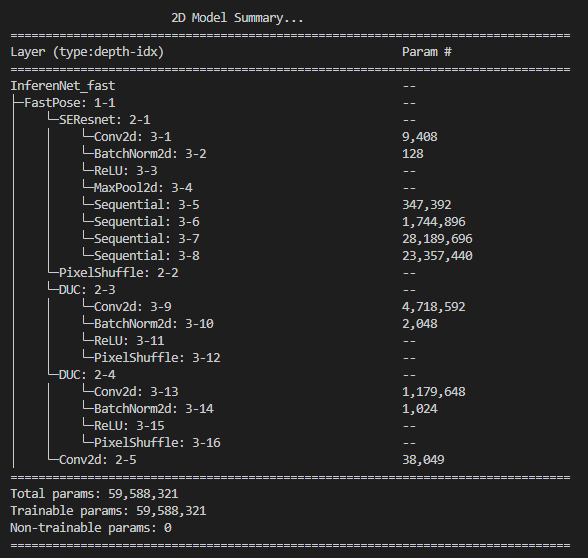
\includegraphics[width=0.7\textwidth]{figures/Implementation/2DModelAr.png}
	\captionsetup{labelformat=empty}
	\caption{2D model summary}
\end{figure}

\pagebreak


\begin{figure}[htp]
    \centering
    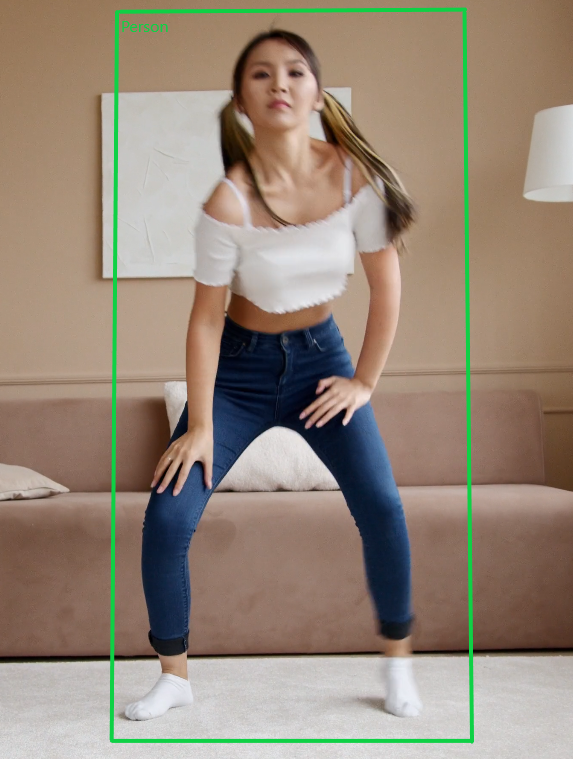
\includegraphics[width=0.4\textwidth]{figures/Implementation/YoloModel.png}%
    \qquad
    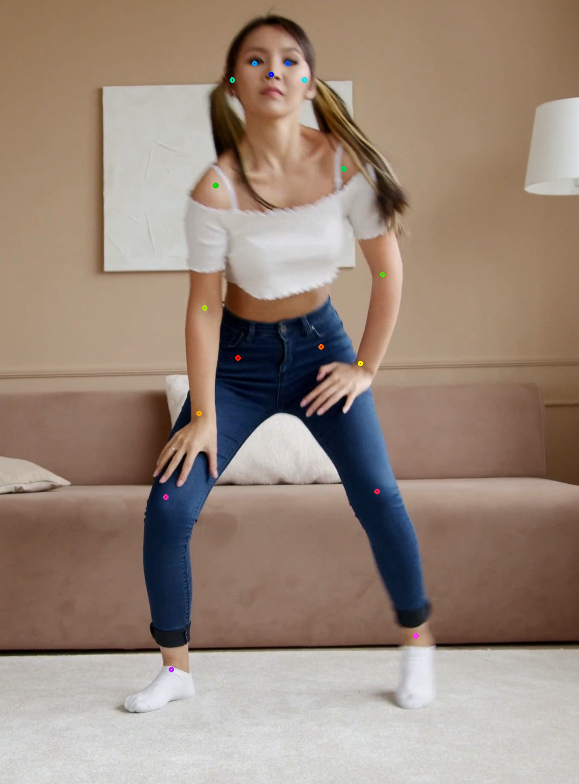
\includegraphics[width=0.4\textwidth]{figures/Implementation/SPPE.png}%
    \qquad
    \captionsetup{labelformat=empty}
    \caption{In the first figure we display the Yolo model Bounding box classification, and in the second the keypoints of the SPPE model}%
\end{figure}


In the above figure, the box estimation is very accurate, but we can see that the keypoints of the model, have a small estimation error on the keypoints that should be symmetrical but are not exactly ( some mm off the right point). We will discuss more about the models estimation errors in the evaluation section.
\subsubsection{2D pose estimation to 3D pose estimation}
The model that we discussed about in the previous section gives us a 2D array (x,y) with 17 keypoints per frame. So, the array's form we have at this moment is (N,17,2) where N is the number of frames. However, we want to work in $R^3$ so we have to estimate the third dimension.  Luckily, for us, there is another pre-trained neural network that can solve this problem. This NN takes as input the array that the AlphaPose model estimated (N,17,2) and tries to predict the third dimension, so it returns a new array with form (N,17,3). However, the accuracy of the estimated third dimension drops significantly. \\


Predicting the 3D joint positions of a human body is defined as the task of 3D human pose estimation. The model we chose estimates the relative 3D position of each joint in relation to the root joint. According to the dataset used (COCO) in the previous estimation, the number of joints $N_j$ is set to 17 in this paper.\\

Human3.6M contains 3.6 million video frames for 11 subjects, of which seven are annotated with 3D poses. Each subject performs 15 actions that are recorded using four synchronized cameras at 50 Hz. In our case, which falls under the category of 2D-to-3D estimation there are two methods by which we could convert the 2D keypoints into 3D. Both methods that we are going to discuss, estimate the 3D pose from the 2D pose, using this as the main dataset as a reference.\\

\subsubsection*{Ground-Truth}

Ground truth represents the desired output of an algorithm on an input. The ground truth would be the ideal output you would hope your algorithm can produce. It is also the standard you are defining, by which you evaluate an algorithm. The closer your algorithm is to ground truth the better.\\

In the context of object tracking, the ground truth would represent the 'true' state of the object in each frame. Typically the state of an object is represented by a bounding rectangle which is defined by a width, height, and center, though you can imagine having a simpler or more complicated state depending on the application.\\

For example, in our case we want to track a human in a video sequence. Therefore the ground-truth is going through each frame of the sequence and determining the bounding rectangle that best encloses the human.\\


\begin{figure}[h]
	\centering
	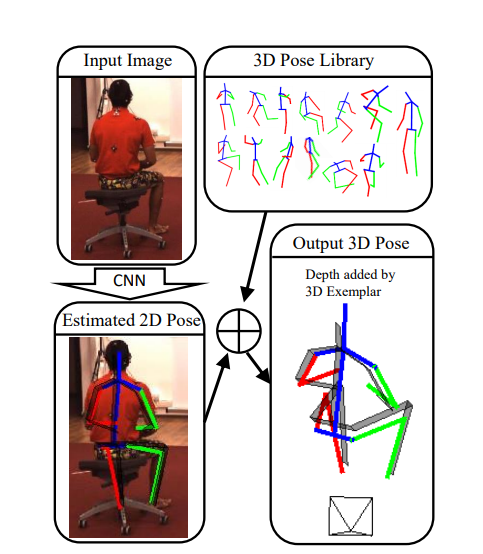
\includegraphics[width=0.75\textwidth]{figures/Implementation/3DModel.png}
	\captionsetup{labelformat=empty}
	\caption{\href{https://arxiv.org/pdf/1811.11742.pdf}
	{The model that takes 2D keypoint sequences (bottom) as input and generates 3D pose
estimates as output (top).}}
\end{figure}


The first method's central idea  \cite{Attention Mechanism Exploits Temporal Contexts: Real-time 3D Human Pose Reconstruction} is to take a sequence of n frames with 2D joint positions as the input and outputs the estimated 3D pose for the target frame as labeled. This model is a fully convolutional architecture with residual connections that takes a sequence of 2D poses as input and transforms them through temporal convolutions.\\

More specifically, this approach does not use heat maps like many other models and instead describes poses with detected keypoint coordinates. This allows the use of efficient 1D convolution over coordinate time series, instead of 2D convolutions over individual heat maps (or 3D convolutions over heat-map sequences). In addition, this idea also makes computational complexity independent of keypoint spatial resolution. This model can reach high accuracy with fewer parameters and allow for faster training and inference. When we loaded the model in our GPU, we used the summary function that is included in the torch library, and it showed that this model has 16,952,371 Trainable parameters. Moreover, we could see the model architecture, in the figure below, again from this function. 


\begin{figure}[h]
	\centering
	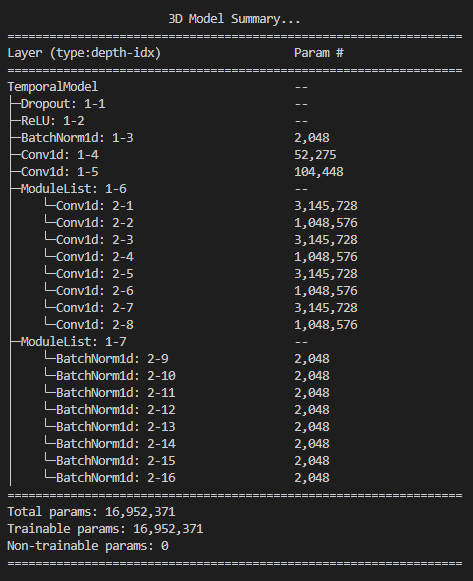
\includegraphics[width=0.6\textwidth]{figures/Implementation/3DModelAr.png}
	\captionsetup{labelformat=empty}
	\caption{3D model summary}
\end{figure}

\pagebreak

\begin{figure}[h]
	\centering
	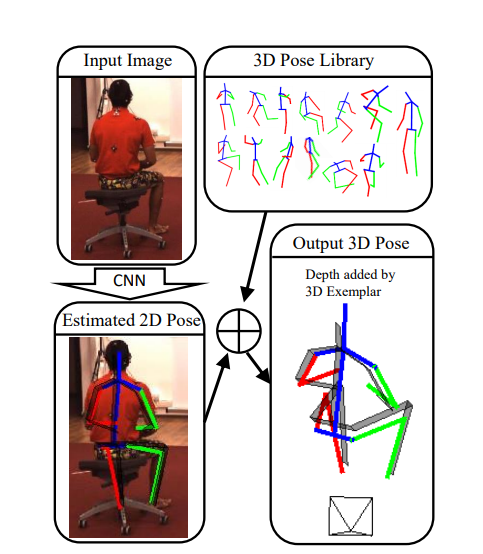
\includegraphics[width=0.65\textwidth]{figures/Implementation/3DModel2Method.png}
	\captionsetup{labelformat=empty}
	\caption{\href{https://arxiv.org/pdf/1612.06524.pdf}
	{3D pose estimation from a 2D estimated pose}}
\end{figure}

The second method's central idea \cite{3D Human Pose Estimation = 2D Pose Estimation + Matching} is to train a neural network to perform 3D pose estimation using both image features from the input image and 2D pose information retrieved from another Neural network (AlphaPose). In other words, this method assumes that the 3D pose X is conditionally independent of the image I, given the 2D pose x, which is not quite true. Given this assumption, we make use of a probabilistic formulation over variables including the image I, the 3D pose $X \in R^{3N}$, and the 2D pose $x \in R^{2N}$ and N is the number of articulated joints. Therefore, we write the joint probability as: 
$$P(X,x,I) = P(X|x) \cdot P(X|I) \cdot P(I)$$
where P(X|I) is a nonlinear function, in our case the AlphaPose model that
predicts the 2D keypoints, and P(X|x) is the Neural network that we will use to estimate the 3D keypoints from the AlphaPose model.\\

Both methods, had great 3D pose reconstruction, while the first method was faster than the second. The first was tested on a single NVIDIA TITAN RTX GPU and for real-time inference, it can reach 3000 FPS, approximately 0.3 milliseconds to process a video frame. In  NVIDIA GeForce GTX 1050 it can reach about 100 FPS, approximately 10 milliseconds to process a video frame. The other method has more complexity since it uses both 2D pose estimation and the image as input. Therefore, the speed was slower, and we decided to choose the faster method since the quality satisfied our needs.\\

So we chose the first model idea, to estimate the 3D human poses from the already estimated 2D. Before this estimation, we normalized all the 2D keypoints. These 2D keypoints were pixels of the image. So we normalized them to have a value between [-1,1] with the below formula:

$$\dfrac{2D_{poses} - \begin{pmatrix} \dfrac{Video_{width}}{2} \ \ ,& \ \dfrac{Video_{height}}{2} \end{pmatrix}}{\begin{pmatrix} \dfrac{Video_{width}}{2} \ \ ,& \ \dfrac{Video_{height}}{2} \end{pmatrix}}$$

Then, after we normalize the 2D poses, we feed them into the model and we get the 3D pose estimation.




\subsubsection{Orientation and Location Estimation}
This whole procedure that we discussed in the previous section, helped us to successfully converted each image of the video that contains only a single person into an array that contains the 3D pose estimation of a human. However, we still are missing something. What we need is the 6D human pose estimation. At this moment we have the knowledge of the orientation of each human bone that our humanoid skeleton has. We have to find the location of the humanoid in the space, which is important if the user wants to apply the root motion to his avatar. A mocap suit estimates the position of each bone in the space, so if we need to match the quality of it we should do the same. However, in our case, the best option was to estimate the location of the parent bone of the human (the hip) and move into space the humanoid according to the hip location. Imagine that our human is moving like a marionette, it can rotate each bone of the body, but the location of the marionette will be according to the actor's hand that is controlling it.\\

Therefore, we came up with a solution to this problem that would help us estimate the human location from a single image. We can use some knowledge that we already have from our models. More specifically, the first model, the 2D human pose estimator, predicts 17 keypoints of the human skeleton, as we have already shown in a figure in the previous sections. In order to estimate the (x,y) of the position we will find the average pixel in the image, between these 17 keypoints. If we do so, this point location should be estimating the human hip position as it is shown in the figure below.

\pagebreak

\begin{figure}[h]
	\centering
	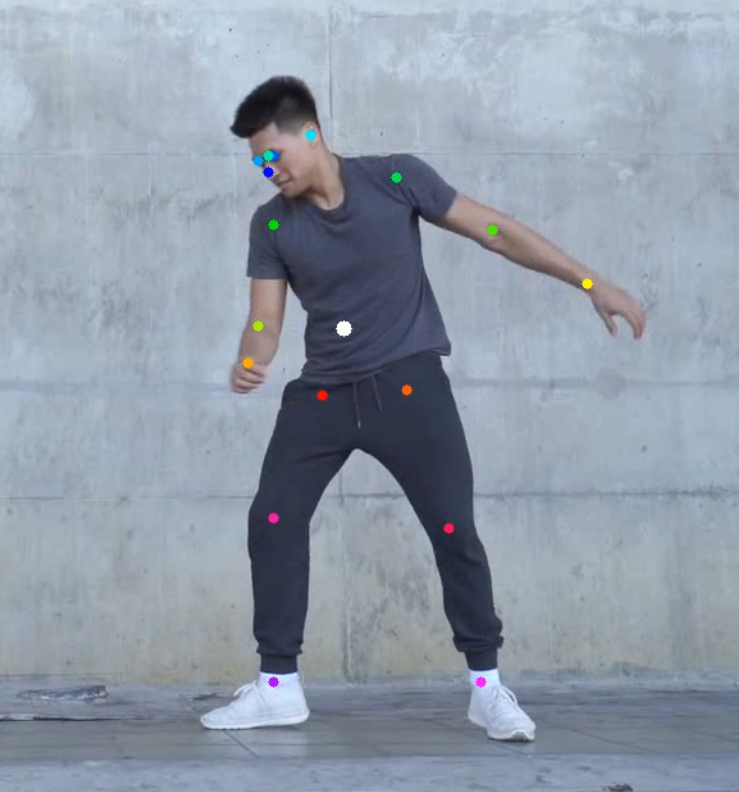
\includegraphics[width=0.65\textwidth]{figures/Implementation/position2D.png}
	\captionsetup{labelformat=empty}
	\caption{\href{https://www.pexels.com/search/videos/dance/}
	{The multi-color keypoints represent the 17 keypoints that the AlphaPose model estimated . The white keypoint is the average of all the estimated keypoints which we will use as the 2D location of the humanoid.}}
\end{figure}

However, we still are missing the Z dimension of the position. Estimating the Depth from a single image is something that many researchers try to solve.Some state-of-the-art works can estimate the 3D location of an object from an image with great accuracy. The most accurate method is to use two cameras to take the image of the object from two different positions. This would minimize the depth error estimation. However, we did not choose this method because it requires two cameras, but we decided to convert the motion of a human from a single video, we wanted our algorithm to be as simpler as it can get for the user.\\

Therefore, the solution that we came up with is very fast O(N) (N is the number of the frames from the input video), but the accuracy in some cases is not great. Again, using the 17 keypoints of the AlphaPose model, we segmented the human inside a box, that contains all the keypoints. In order to estimate the depth of the image, we calculate the $log(area)_2$ of this box, and we normalize this number depending on the video resolution. Due to the log, small changes due to some limb motion do not affect the results. The animators can fix some errors in the humanoid position later, but we will also offer a tool that will help them in this procedure. In the figure below we can the human box segmentation.

\begin{figure}[h]
	\centering
	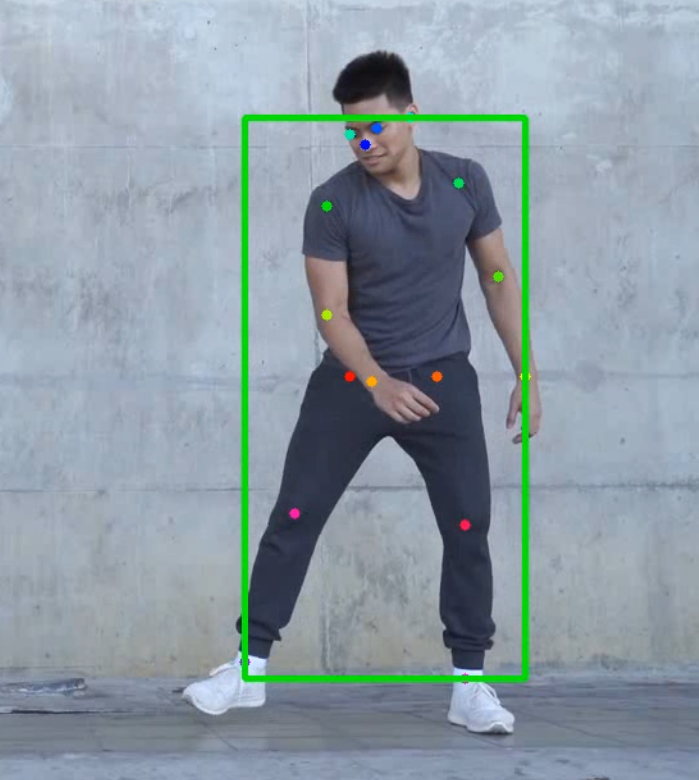
\includegraphics[width=0.65\textwidth]{figures/Implementation/position3D.png}
	\captionsetup{labelformat=empty}
	\caption{\href{https://www.pexels.com/search/videos/dance/}
	{Human Segmentation using the 17 keypoints from AlphaPose model}}
\end{figure}


\subsubsection{3D Pose to Biovision Hierarchical (BVH)}

We have to convert the pose that we managed to estimate, into a file that animator software can read. We choose to convert it into a BVH file, as it is the most common file for computerized mocap clips. \\

Firstly, we have to create a skeleton in BVH form. This skeleton must be identical to the skeleton of the datasets that our model used. Therefore we created in python a skeleton with 17 main bones and 4 limb bones that follow the movement of their parent bone. We also initialized the first frame of the movement as a T-Pose, to make the motion retarget easier for the animators.\\

In the BVH format, the following relationship holds between the joints:
$$orientation_j=R_{P(j)}offset_j + orientation_{P(j)}$$

where $orientation_j$ indicates the 3D orientation of joint j, P(j) returns the parent of joint j in whatever DAG (directed acyclic graph) the orientations are modeled in (generally the DAG starts at the root and points towards the end-effectors) $offset_j$ indicates the offset of joint j relative to its parent P(j) (aka the connecting limb), and $R_{P(j)}$ is the 3D rotation that determines how much should $offset_j$ be rotated from an initial pose (generally a T-pose). In the BVH format, for each parent P(j), we need to store $R^{-1}_{P(j)}R_j$. The main problem was working with joints that had multiple children, for example, the root joint, which has connections to both legs as well as the spine. Therefore, we came up with a solution for joints with multiple children, I had to make copies with offset=0, and assign those as parents of the corresponding chains. \\

Regarding the position of the humanoid, which in our case only only the hip has, we can easily convert it. We assume that the hip starts in the frame 0 in the location (0, hipSkeletonHeight, 0) , so with this point as a reference, we can perfectly convert the position into an computerized space that the animators will use.\\

\begin{figure}[htp]
    \centering
    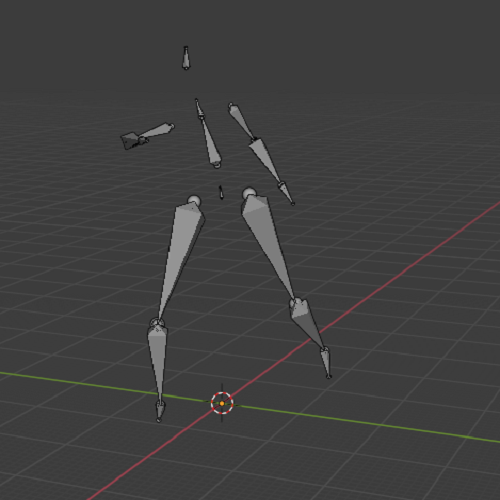
\includegraphics[width=5cm]{figures/Implementation/skeleton1.png}%
    \qquad
    \includegraphics[width=5cm]{figures/Implementation/skeleton2.png}%
    \qquad
    \includegraphics[width=5cm]{figures/Implementation/skeleton3.png}%
    \qquad
    \includegraphics[width=5cm]{figures/Implementation/skeleton4.png}%
    \captionsetup{labelformat=empty}
    \caption{The results of the BVH File from a video when we import it into Blender. The same frame from different camera positions.}%
    \label{fig:example}%
\end{figure}

Finally, we completed the first phase of our goal, we estimated the 6D human pose, or we estimated the orientation and the location of the human in the video for each frame and we convert it into a BVH file. Subsequently, we will discuss about some ways that will improve these results 



\subsection{Animator Tools}
In this section, we will propose some tools for the animators that will help them process and edit further the BVH file that we created. We created three tools for the animators. The first allows the user to amplify each dimension of the position speed for all the frames. In the second tool, we used some digital and Gaussian distribution filters in order to smooth out the BVH motion data that the neural networks estimated from the video, which help to reduce the noise between each frame. Finally, we created a tool that converts the bvh motion data into a mp4 video. More specifically, we created a 3D space, and we import each joint of the motion as a point for each frame. We will discuss later in this section more thoroughly about this visualization method.
\subsubsection{Biovision Hierarchical (BVH)}
The BVH file format was originally developed by Biovision, a motion capture services company, as a way to provide motion capture data to their customers. The name BVH stands for Biovision hierarchical data. This format mostly replaced an earlier format that they developed, the BVA format, as a way to provide skeleton hierarchy information in addition to the motion data. The BVH format is an excellent all-around format, its only drawback is the lack of a full definition of the basis pose (this format has only translational offsets of children segments from their parent, no rotational offset is defined), it also lacks explicit information for how to draw the segments but that has no bearing on the definition of the motion.\\

A BVH file has two parts, a header section that describes the hierarchy and initial pose of the skeleton; and a data section that contains the motion data. The start of the header section begins with the keyword "HIERARCHY". The following line starts with the keyword "ROOT" followed by the name of the root segment of the hierarchy to be defined. After this hierarchy is described it is permissible to define another hierarchy, this too would be denoted by the keyword "ROOT". In principle, a BVH file may contain any number of skeleton hierarchies. In practice the number of segments is limited by the format of the motion section, one sample in time for all segments is on one line of data and this will cause problems for readers which assume a limit to the size of a line in a file.\\

The BVH format now becomes a recursive definition. Each segment of the hierarchy contains some data relevant to just that segment then it recursively defines its children. The line following the ROOT keyword contains a single left curly brace '\{', the brace is lined up with the "ROOT" keyword. The line following a curly brace is indented by one tab character, these indentations are mostly to just make the file more human-readable but some BVH file parsers expect the tabs. The first piece of information about a segment is the offset of that segment from its parent, or in the case of the root object, the offset will generally be zero. The offset is specified by the keyword "OFFSET" followed by the X, Y, and Z offset of the segment from its parent. The offset information also indicates the length and direction used for drawing the parent segment. In the BVH format, there isn't any explicit information about how a segment should be drawn. This is usually inferred from the offset of the first child defined for the parent. Typically, only the root and the upper body segments will have multiple children.\\

The line following the offset contains the channel header information. This has the "CHANNELS" keyword followed by a number indicating the number of channels and then a list of that many labels indicating the type of each channel. The BVH file reader must keep track of the channel count and the types of channels encountered as the hierarchy information is parsed. Later, when the motion information is parsed, this ordering will be needed to parse each line of motion data. This format appears to have the flexibility to allow for segments that have any number of channels that can appear in any order.\\

You can see that the order of the rotation channels appears a bit odd, it goes Z rotation, followed by the X rotation, and finally the Y rotation. On the line of data following the specification of the channel, there can be one of two keywords, either you will find the "JOINT" keyword or you will see the "End Site" keyword. A joint definition is identical to the root definition except for the number of channels. This is where the recursion takes place, the rest of the parsing of the joint information proceeds just like a root. The end site information ends the recursion and indicates that the current segment is an end effector (has no children). The end site definition provides one more bit of information, it gives the length of the preceding segment just like the offset of a child defines the length and direction of its parent's segment. The end of any joint, end site, or root definition is denoted by a right curly brace '\}'. This curly brace is lined up with its corresponding right curly brace.\\

The motion section begins with the keyword "MOTION" on a line by itself. This line is followed by a line indicating the number of frames, this line uses the "Frames:" keyword (the colon is part of the keyword) and a number indicating the number of frames, or motion samples that are in the file. On the line after the frame definition is the "Frame Time:" definition, this indicates the sampling rate of the data. The rest of the file contains the actual motion data. Each line is one sample of motion data. The numbers appear in the order of the channel specifications as the skeleton hierarchy was parsed. In the figure below, we can see the hierarchy as well as the motion format of our Skeleton that we discussed in this section.


\begin{figure}[htp]
    \centering
    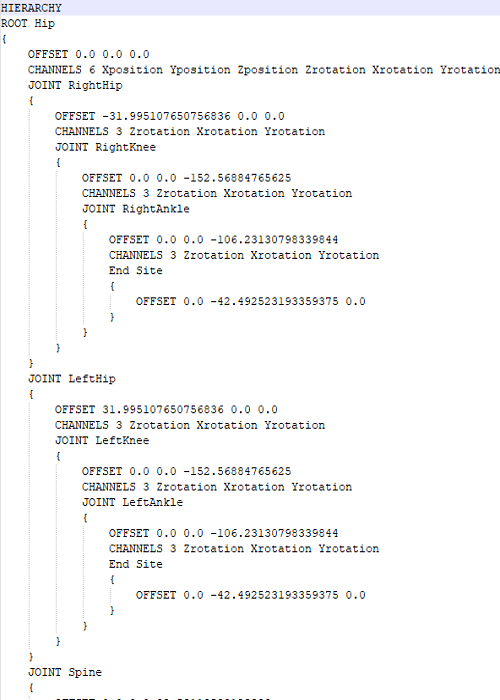
\includegraphics[width=6.5cm]{figures/Implementation/bvh1.png}%
    \qquad
    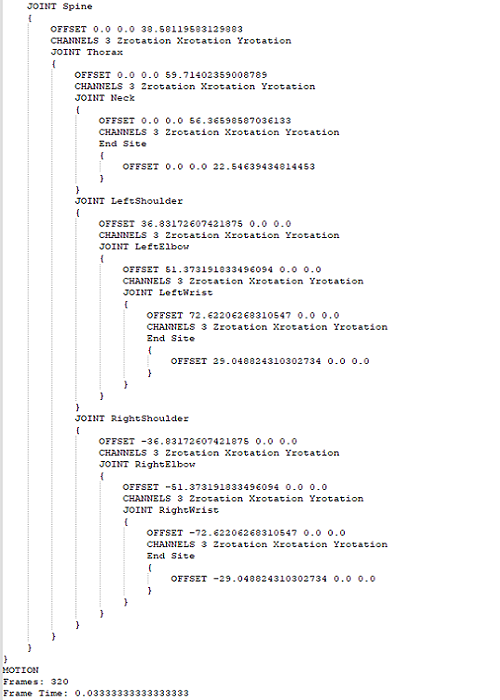
\includegraphics[width=6.5cm]{figures/Implementation/bvh2.png}%
    \qquad
    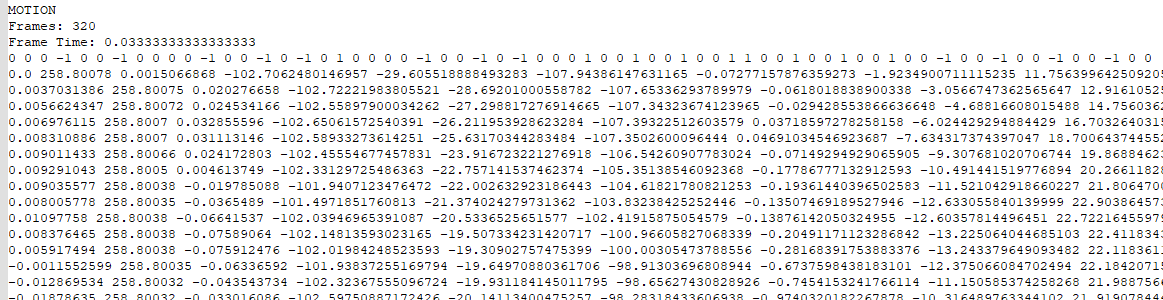
\includegraphics[width=1\textwidth]{figures/Implementation/bvh3.png}%
    \captionsetup{labelformat=empty}
    \caption{BVH format of the motion and hierarchy for the Skeleton that we are using. The first line of the motion, sets the skeleton in T-Pose and the rest contain the motion data.}
\end{figure}


\subsubsection{BVH Position Tool Editing}
Unfortunately, the method of the skeleton position estimation, in some cases may do not satisfy the animators. Therefore, the purpose of this tool is to allow the animator to make some adjustments of his preference in the motion root of the skeleton. More specifically, the animator will input three float numbers one for each dimension, that will multiply for the correspond position of the hip for each frame of the motion data. This will amplify the motion root speed if the float number is above one , otherwise it will decreased it. One last note is that the Skeleton initial height is in the ground, therefore we do not recommend to amplify the Y dimension of the Skeleton, since the Skeleton will float into the 3D space. 
\subsubsection{BVH Noise Filtering}
The Neural Networks that we are using, and generally all the neural networks that estimate or generate something have an error rate, in our case, a missing rate from the real target. More specifically, our Neural Networks may falsie estimate some millimeter or centimeter from the real location of that keypoint. That may happen for each keypoint that they try to estimate for every frame. And every estimation is completely undependable from another. Therefore, this produces a type of noise through the motion data, that can be clearly seen even in our video mp4 player (for better visualization use Blender or another 3D computer graphics software tool-set). \\

The animators could reduce this noise by hand, correcting each joint location and orientation for each frame. This procedure is what is happening, even with mocap suits when the animators want to create flawlessly motion data. However, this procedure is clearly too time-consuming, since a video may contain over 1000 frames and each frame contains 17 joints with three or six dimensions each.\\

Therefore, we came up with a solution that will significantly reduce this noise. It may need some further editing from the animators, but we will save them again plenty of time. The best way to reduce the noise is to filter out with smoothing filter the motion data. We offer to the animators three different filters, the Mean, the Gaussian, and the Butterworth. \\

These filters are three well-known filters that many researchers use to reduce the noise from images. In our case, we want to remove the noise from the motion data. The form of the motion data is a 2D array, that has the same properties as an image. However, the fact that the motion data has the form of an image, is not the only reason that we can use these filters. It is that for every keypoint of the motion data, some of its neighbors have a dependence on it. For example, the keypoints of a bone have a dependence on their neighbor frames. This also happens in the images, every pixel has a dependent on some of its neighbors in order to create some shapes and objects.

\subsubsection*{Mean Filter}
Mean filtering \cite{Mean Filtering} is a simple, intuitive and easy to implement method of smoothing images, i.e. reducing the amount of intensity variation between one pixel and the next. It is often used to reduce noise in images. So we decided to use this to filter the noise from the motion data, imagine that each frame has a similar form of an image, however it is more sensitive to the noise.\\

The idea of mean filtering is simply to replace each pixel value in an image with the mean ('average') value of its neighbors, including itself. This has the effect of eliminating pixel values which are unrepresentative of their surroundings. Mean filtering is usually thought of as a convolution filter. Like other convolutions it is based around a kernel, which represents the shape and size of the neighborhood to be sampled when calculating the mean. Often a 3x3 square kernel is used, as shown in the figure below, although larger kernels (e.g. 5x5 squares, it has to be an odd number) can be used for more severe smoothing. (Note that a small kernel can be applied more than once in order to produce a similar but not identical effect as a single pass with a large kernel.)


\begin{figure}[h]
	\centering
	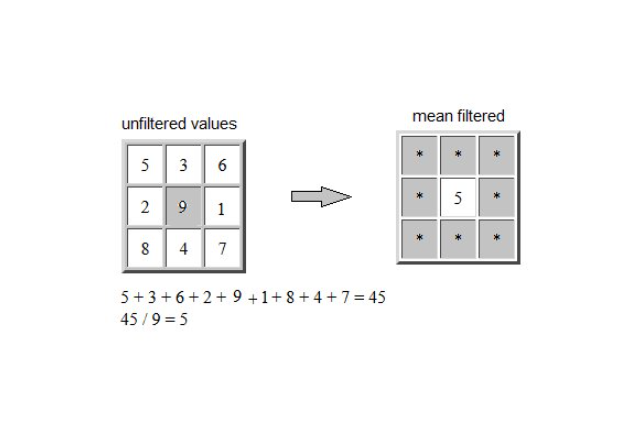
\includegraphics[width=1\textwidth]{figures/Implementation/meanFilter.png}
	\captionsetup{labelformat=empty}
	\caption{\href{https://www.researchgate.net/publication/348548607_The_Challenge_of_Predicting_OAG_Progression_from_the_Initial_Visual_Field_Test/figures?lo=1}
	{Mean Filter procedure with a 3x3 kernel}}
\end{figure}

In general, the Mean filter allows a great deal of high spatial frequency detail to pass while remaining very effective at removing noise on images where less than half of the pixels in a smoothing neighborhood have been effected. (As a consequence of this, mean filtering can be less effective at removing noise from images corrupted with Gaussian noise.)\\

One of the major problems with the mean filter is that it is relatively expensive and complex to compute. To find the mean it is necessary to sort all the values in the neighborhood into numerical order and this is relatively slow, even with fast sorting algorithms such as quicksort (it has an average complexity of O(log(N)) and in worst case O($N^2$)). The basic algorithm can, however,be enhanced somewhat for speed. A common technique is to notice that when the neighborhood window is slid across the image, many of the pixels in the window are the same from one step to the next, and the relative ordering of these with each other will obviously not have changed. Clever algorithms make use of this to improve performance.\\

In our algorithm, we ask the animator to give us the size of the kernel that he wants to use in order to filter the motion data. We suggest they use a kernel with a size smaller than 9x9, but they are free to use whatever they want that will increase the quality of the motion data and decrease their further editing on it.

\subsubsection*{Gaussian Filter}
The Gaussian smoothing operator is a 2-D convolution operator that is used to 'blur' images and remove detail and noise. In this sense it is similar to the mean filter, but it uses a different kernel that represents the shape of a Gaussian ('bell-shaped') hump. This kernel has some special properties which are detailed below.\\
The Gaussian distribution in 1-D has the form:
$$ G(x) = \dfrac{1}{\sqrt{2\pi\sigma}} e^{-\dfrac{(x-\mu)^2}{2\sigma^2}}$$

where $\sigma$ is the standard deviation of the distribution. We have also assumed that the distribution has a mean of zero (i.e. it is centered on the line x=0). 

\begin{figure}[h]
	\centering
	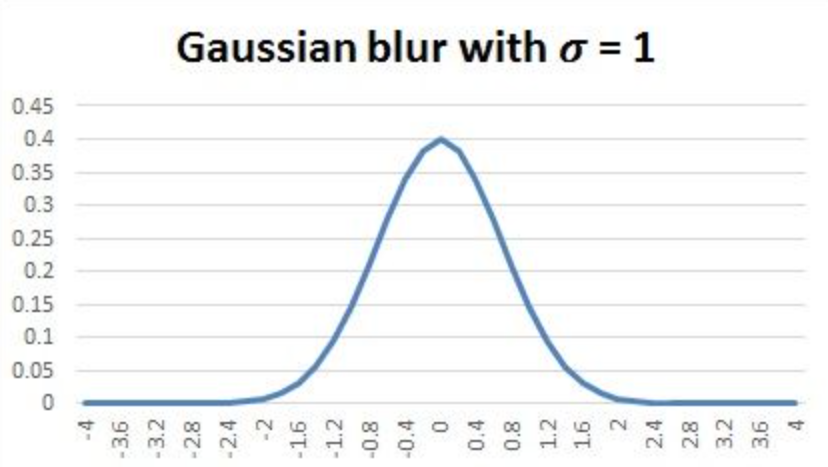
\includegraphics[width=1\textwidth]{figures/Implementation/Gaussian1D.png}
	\captionsetup{labelformat=empty}
	\caption{\href{https://fiveko.com/assets/pics/math/gauss1d_shape.jpg}
	{ 1-D Gaussian distribution with mean 0 and $\sigma$=1}}
\end{figure}

In our case we need a 2-D Gaussian Filter. Therefore, the idea of Gaussian smoothing is to use this 2-D distribution as a `point-spread' function, and this is achieved by convolution. Since the image is stored as a collection of discrete pixels we need to produce a discrete approximation to the Gaussian function before we can perform the convolution. In theory, the Gaussian distribution is non-zero everywhere, which would require an infinitely large convolution kernel, but in practice it is effectively zero more than about three standard deviations from the mean, and so we can truncate the kernel at this point. Figure 3 shows a suitable integer-valued convolution kernel that approximates a Gaussian with a $\sigma$ of 1.0. It is not obvious how to pick the values of the mask to approximate a Gaussian. One could use the value of the Gaussian at the centre of a pixel in the mask, but this is not accurate because the value of the Gaussian varies non-linearly across the pixel.\\

Once a suitable kernel has been calculated, then the Gaussian smoothing can be performed using standard convolution methods. The convolution can in fact be performed fairly quickly since the equation for the 2-D isotropic Gaussian shown above is separable into x and y components. Thus the 2-D convolution can be performed by first convolving with a 1-D Gaussian in the x direction, and then convolving with another 1-D Gaussian in the y direction. (The Gaussian is in fact the only completely circularly symmetric operator which can be decomposed in such a way.) \\



The Gaussian distribution in 2-D has the form:

$$ G(x,y) = \dfrac{1}{\sqrt{2\pi\sigma}} e^{-\dfrac{(x-\mu)^2 + (y-\mu)^2}{2\sigma^2}}$$\\

\pagebreak

\begin{figure}[h]
	\centering
	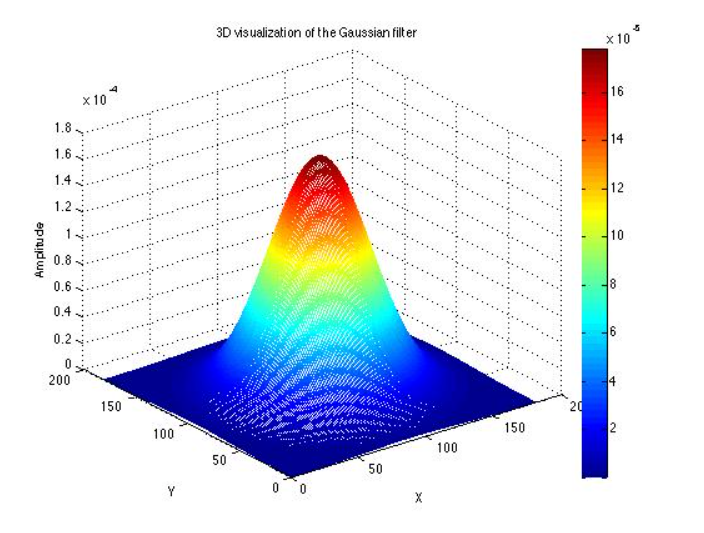
\includegraphics[width=1\textwidth]{figures/Implementation/Gaussian2D.png}
	\captionsetup{labelformat=empty}
	\caption{\href{https://stackoverflow.com/questions/23981437/visualization-of-gaussian-laplacian-etc-filters-in-matlab}
	{2-D Gaussian distribution with mean 0 and $\sigma$=1}}
\end{figure}

The effect of Gaussian smoothing is to blur an image, in a similar fashion to the mean filter. The degree of smoothing is determined by the standard deviation of the Gaussian. (Larger standard deviation Gaussian's, of course, require larger convolution kernels in order to be accurately represented.)\\

The Gaussian outputs a "weighted average" of each pixel's neighborhood, with the average weighted more towards the value of the central pixels. This is in contrast to the mean filter's uniformly weighted average. Because of this, a Gaussian provides gentler smoothing and preserves edges better than a similarly sized mean filter.\\

One of the principle justifications for using the Gaussian as a smoothing filter is due to its frequency response. Most convolution-based smoothing filters act as low-pass frequency filters. This means that their effect is to remove high spatial frequency components from an image. The frequency response of a convolution filter, i.e. its effect on different spatial frequencies, can be seen by taking the Fourier transform of the filter.\\

Both filters attenuate high frequencies more than low frequencies, but the mean filter exhibits oscillations in its frequency response. The Gaussian on the other hand shows no oscillations. In fact, the shape of the frequency response curve is itself (half a) Gaussian. So by choosing an appropriately sized Gaussian filter we can be fairly confident about what range of spatial frequencies are still present in the image after filtering, which is not the case of the mean filter. This has consequences for some edge detection techniques, as mentioned in the section on zero crossings. (The Gaussian filter also turns out to be very similar to the optimal smoothing filter for edge detection under the criteria used to derive the Canny edge detector.)\\

In our algorithm, we ask the animator to give us the standard deviation of the distribution, (the $\sigma$) as well as the border( the mean value $\mu$) in order to filter the motion data. Gaussian filter differs, what happens is to make each frame of the motion data less sharp and more united between the neighbor frames. Therefore, each motion data may have a unique ideal standard deviation of the distribution and border that the animators have to find by hand.

 
\subsubsection*{Butterworth Filter}
The first two filter were digital filters that many researchers use to clear the noise from images. We used them to clear the noise from the motion data, which works in our case due to some similarities that there are in images and our motion data. In this point, we propose another different type of filter that can also clear our motion data noise. \\

\begin{figure}[h]
	\centering
	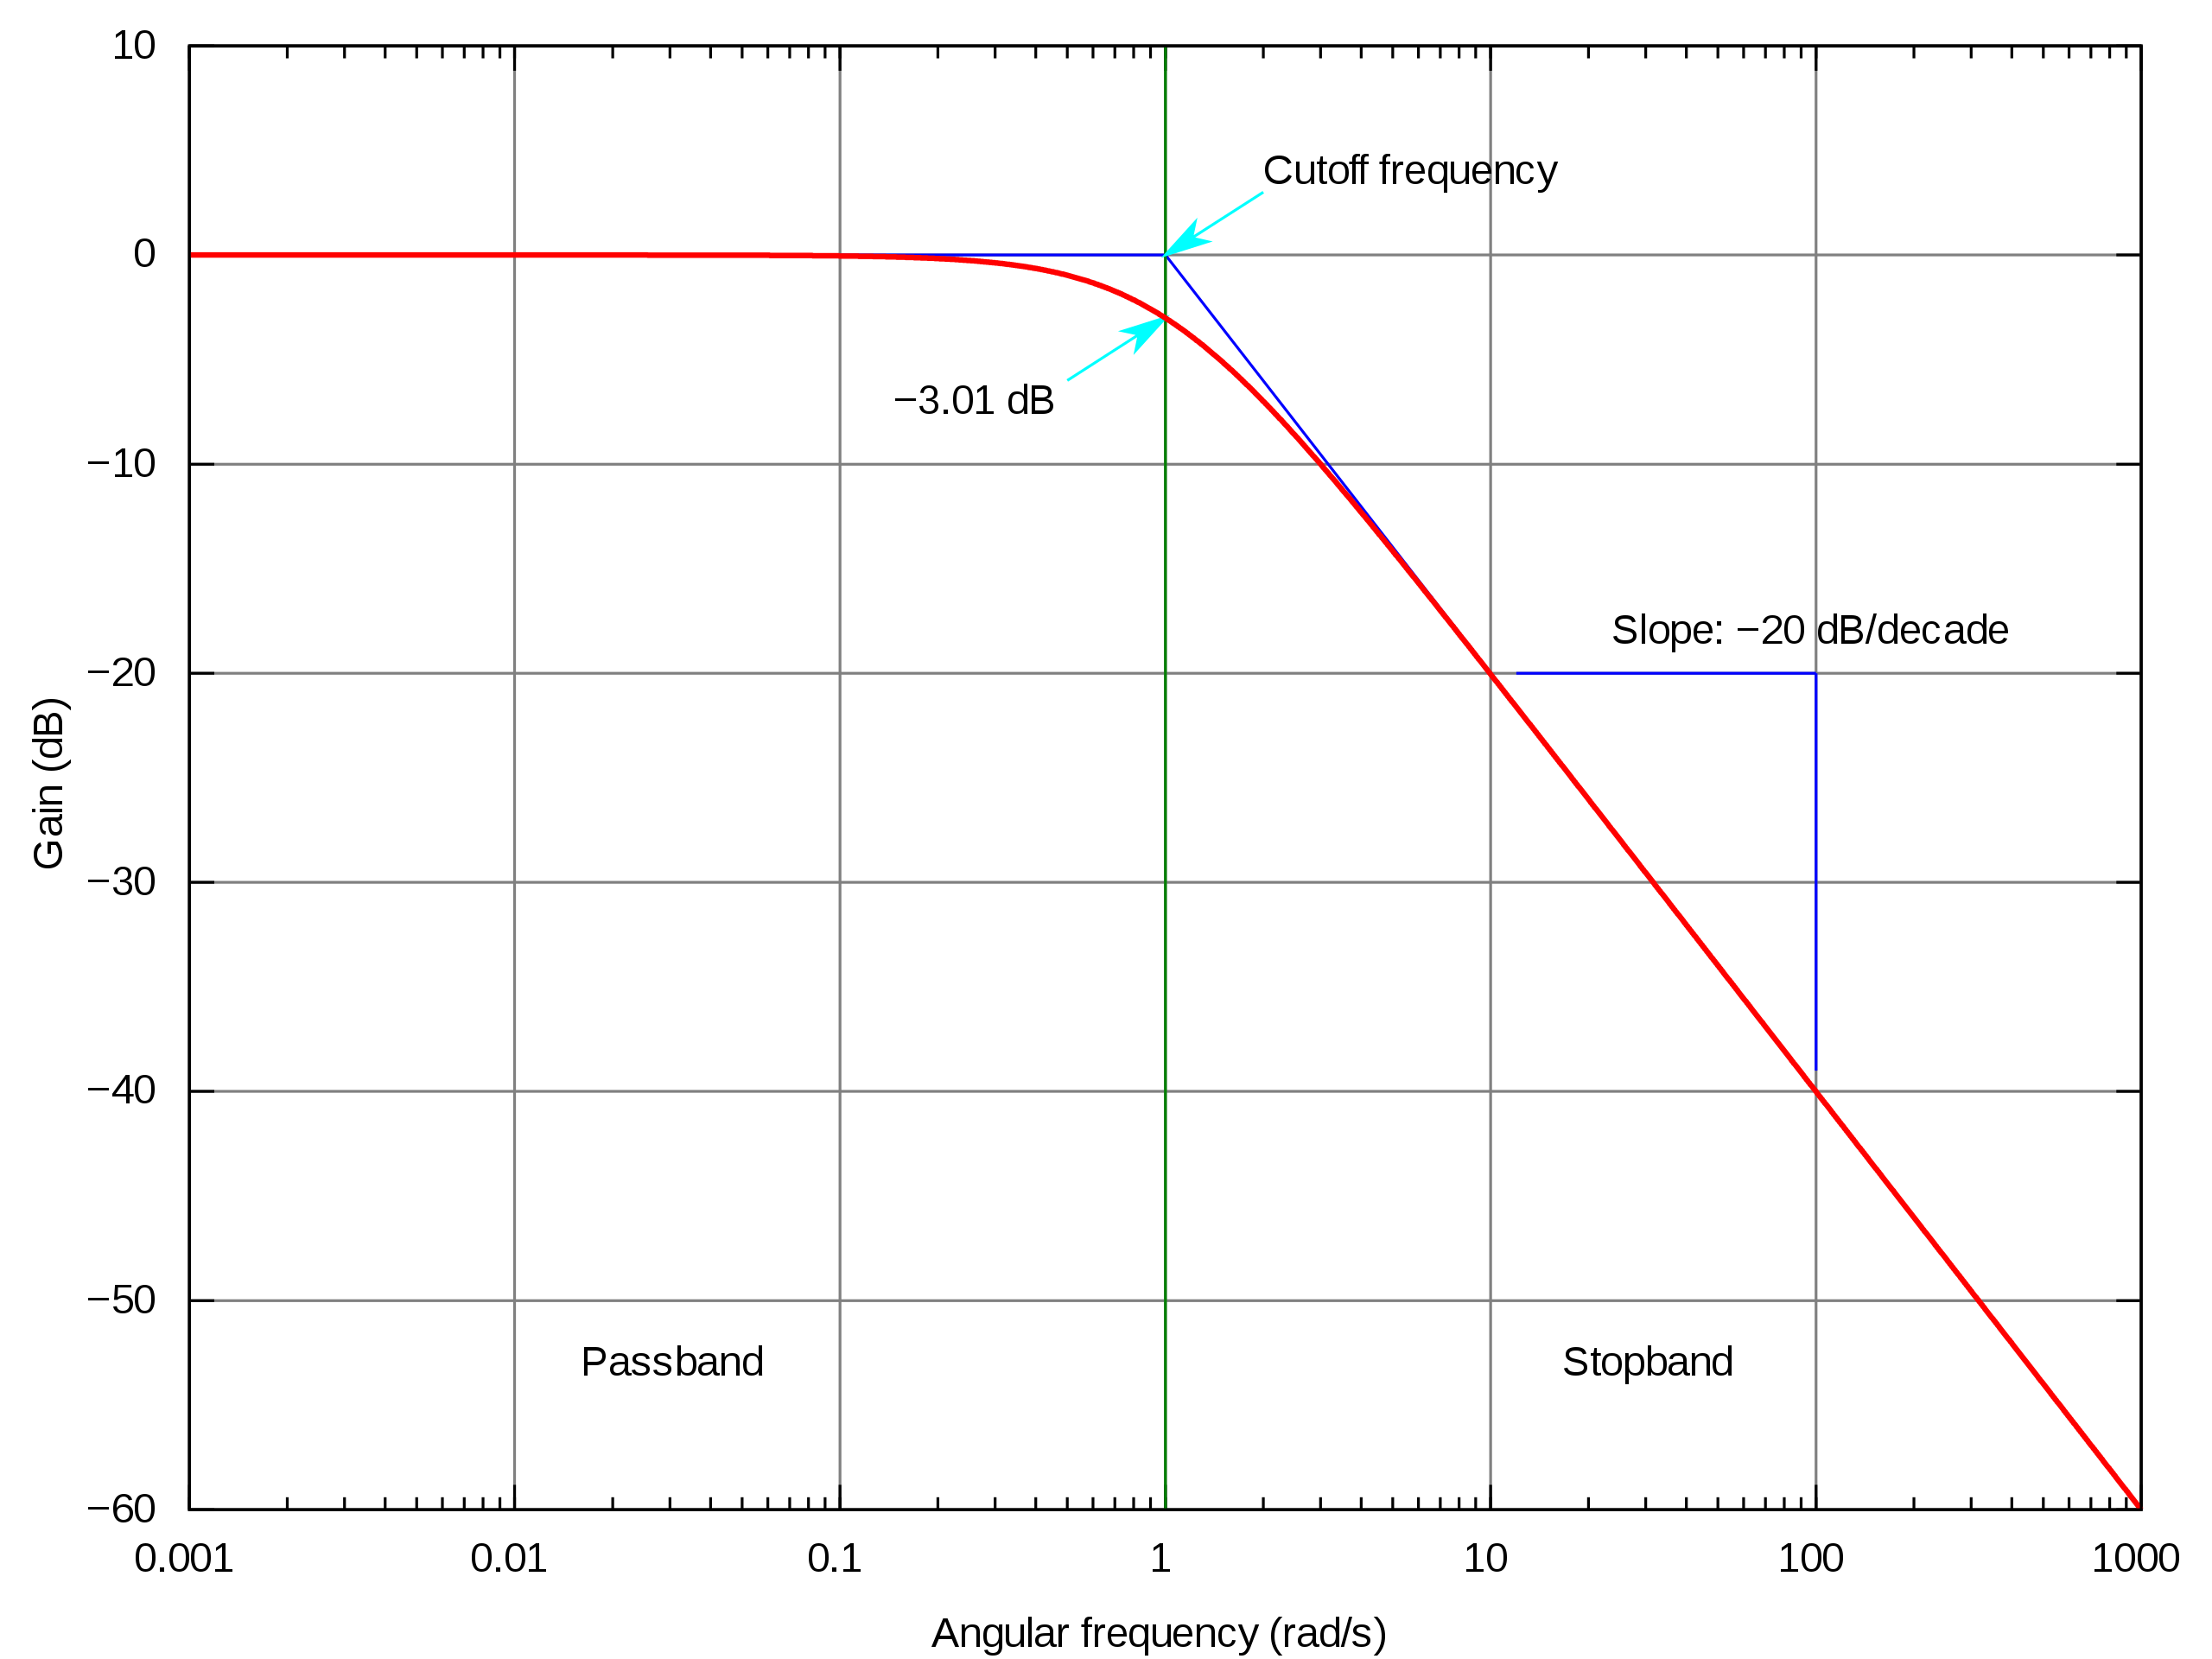
\includegraphics[width=0.7\textwidth]{figures/Implementation/butterworthfilter.png}
	\captionsetup{labelformat=empty}
	\caption{\href{https://upload.wikimedia.org/wikipedia/commons/thumb/6/60/Butterworth_response.svg/2560px-Butterworth_response.svg.png}
	{A low-pass Butterworth Filter}}
\end{figure}

The Butterworth filter is a type of signal processing filter designed to have as flat frequency
response as possible (no ripples) in the pass-band and zero roll off response in the stop-band.
Butterworth filters are one of the most commonly used digital filters in motion analysis and in
audio circuits. They are fast and simple to use. Since they are frequency-based, the effect of
filtering can be easily understood and predicted. Choosing a cutoff frequency is easier
than estimating the error involved in the raw data in the spline methods. However, one main
disadvantage of the Butterworth filter is that it achieves this pass band flatness at the expense
of a wide transition band as the filter changes from the pass band to the stop band. It also has
poor phase characteristics as well. The ideal frequency response, referred to as a "brick wall"
filter in the figure below.

\begin{figure}[h]
	\centering
	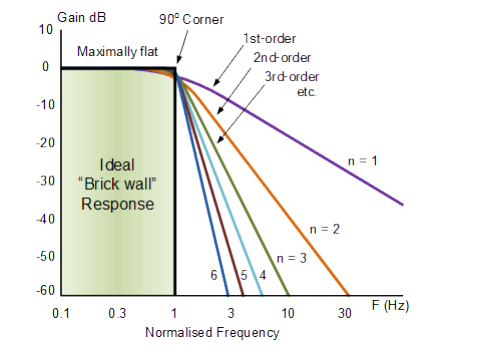
\includegraphics[width=1\textwidth]{figures/Implementation/butterworth.png}
	\captionsetup{labelformat=empty}
	\caption{\href{https://www.electronics-tutorials.ws/wp-content/uploads/2018/05/filter-fil57.gif}
	{Ideal Frequency Response for a low-pass Butterworth Filter}}
\end{figure}

The higher the Butterworth filter order, the higher the number of cascaded stages
there are within the filter design, and the closer the filter becomes to the ideal "brick wall"
response. However, in practice this "ideal" frequency response is unattainable as it produces
excessive pass-band ripple. The generalised equation representing a "nth" Order Butterworth filter, the frequency response is given as:

$$H_{(j\omega)} = \dfrac{1}{\sqrt{1 + \epsilon^2 (\dfrac{\omega}{\omega_p})^{2n}}}$$

Where: n represents the filter order, Omega $\omega$ is equal to $2\pi f$ and Epsilon $\epsilon$ is the maximum pass band gain, ($A_{max}$). If $A_{max}$ is defined at a frequency equal to the cut-off -3dB corner point ($f_c$), $\epsilon$ will then be equal to one and therefore $\epsilon^2$ will also be one. So we simplify the above equation, supposing that we have $A_{max}$ or $\dfrac{H_0}{H_1} = \sqrt{2}$ which means that the cut-off frequency is at -3dB, where $H_0$ is the Maximum Pass band Gain and $H_1$ the Minimum Pass band Gain.\\


In our algorithm, we ask the animator to give us the cut-off frequency , (the $\omega$), the order n of the butterworth filter as well as the fast Fourier transform  border in order to filter the motion data.\\

These are the three filters that we use to clean the noise from the motion data. To compare these filters someone must run the algorithm, since the output of the cleaning is a sequence of motion, and it is impossible to upload a video to represent it in this presentation. Nevertheless, all three of them can clean the majority of the noise that neural networks generate in the motion data, without affecting the motion information.
\subsubsection{BVH Video Player}
We also created a tool that gives the option to the animators to display the results of the BVH files into a panel in the form of an mp4. In particular, we convert the information that we get from the motion data into an mp4, and then we display it to the user.  This procedure is quite simple. We read from the BVH file the Skeleton information, as well as the motion data. We use the matplotlib library that allows us to create a 3D space, and we import into that space all the keypoints for each frame. Therefore, we have completed our algorithm. The animators can convert any human video that meets our requirements into a BVH file. Then they can clear the motion data, with the tool that we are offering, and afterward render the animation into an avatar in order to import it to a Game Engine like Unity.  In the figure below someone can see the input video that someone wants to extract the motion compared to the visualization that we created, the visualization that Blender offers, and finally the motion inside a Game Engine when it is rendered into a humanoid avatar.

\pagebreak

\begin{figure}[htp]
    \centering
    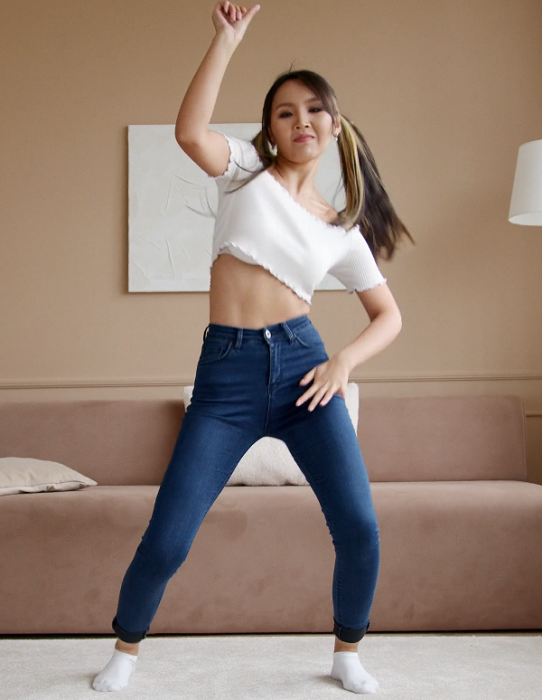
\includegraphics[width=0.35\textwidth]{figures/Implementation/videoplayer1.png}%
    \qquad
    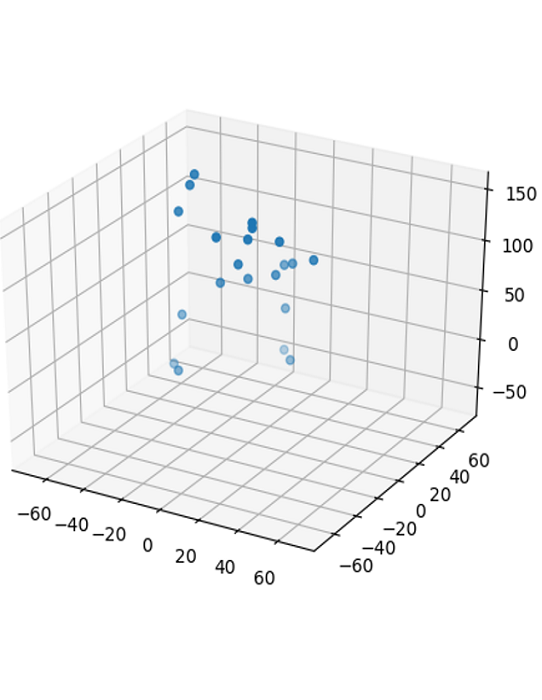
\includegraphics[width=0.35\textwidth]{figures/Implementation/videoplayer2.png}%
    \qquad
    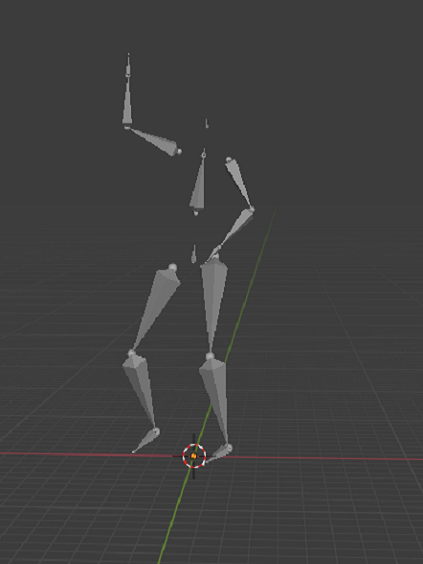
\includegraphics[width=0.35\textwidth]{figures/Implementation/videoplayer3.png}%
    \qquad
    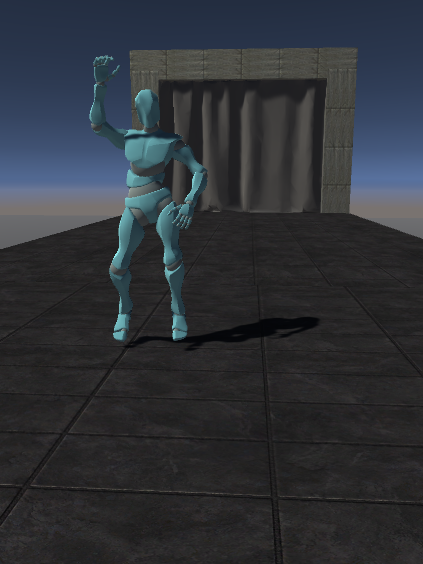
\includegraphics[width=0.35\textwidth]{figures/Implementation/videoplayer4.png}%
    \captionsetup{labelformat=empty}
    \caption{We display a frame from the input video, and the estimated BVH file, in both our video player and Blender. Finally, we display the BVH file when we clean it, convert it into an FBX file, and import it to Unity.}%
\end{figure}

\subsubsection*{Rendering an Avatar to the BVH file}

At this point, we completed the second phase of this Thesis. The final phase is to create a more friendly environment for the user that will use these algorithms and tools. The last image of the above figure is the desired output that we want, the FBX file. This file is the BVH file that we created when we render it into an avatar. More specifically, the FBX file, in our case, is a motioned BVH Skeleton with humanoid skin. Someone can find these skins on some online websites, like mixamo, that's where we got the skin in that image, or he can create his own avatar in studios like Blender. There are some other online applications where someone can find an avatar like Polycom, it is an application that allows you to create high-quality 3D models from photos with any mobile phone. For a Humanoid 3D model it may need many photos but someone can create an avatar that looks like himself, and if we combine it with our thesis, someone can convert his real-life motion into a computerized humanoid avatar that has his form and motion.
\subsection{Windows Application}
In the previous chapters, we discussed about our algorithms and the tools that we offer to the animators. However, the environment that someone has to use in order to run these algorithms is not very friendly to the users. If someone does not have excellent knowledge of python and at least the basic knowledge of Neural Networks, then may struggle to run the raw python code.\\

Therefore, we converted the raw python code into a Windows Application that run all the aspects of the code. Firstly, the User will convert the real Video with a Human motion that meets our requirements into a BVH file, and afterwards he will use our tool to visualize, clean and edit the motion data that our algorithms estimated. \\

Notice that these BVH files can be only imported to 3D computer graphics software tool sets (Maya, Blender, Motion Builder, etc.). If the user wants to import them into a Game Engine (Unity, Unreal Engine, etc.) he must convert this file into an FBX file. An FBX (.FBX) file is a format used to exchange 3D geometry and animation data. All the 3D computer graphics software tool-sets which we mentioned, can easily and fast convert every BVH file into an FBX.
\subsubsection{Tkinter Library}
Converting a raw Python code into a Windows Application, can not be done in many different ways. The way that we chose to follow is to use the Tkinter Python library. Tkinter is the standard GUI library for Python. Python when combined with Tkinter provides a fast and easy way to create GUI applications. This Python framework provides an interface to the Tk toolkit and works as a thin object-oriented layer on top of Tk. The Tk toolkit is a cross-platform collection of  'graphical control elements', aka widgets, for building application interfaces.\\

Many people may think that this library will reduce the raw python performance. At first glance, it is reasonable to assume that Tkinter is not going to perform well. While this opinion is true, in modern systems it really does not matter too much.\\

Tkinter (Tk) consists of a number of modules \cite{Tkinter 1,Tkinter 2}. The Tk interface is located in a binary module named \_tkinter (this was Tkinter in earlier versions). This module contains the low-level interface to Tk, and should never be used directly by application programmers. It is usually a shared library (or DLL), but might in some cases be statically linked with the Python interpreter. In addition to the Tk interface module, Tkinter includes a number of Python modules. The two most important modules are the Tkinter module itself, and a module called Tkconstants.\\

The main goal is to create a .exe file that the user will open in order to run this Application. There is a library in python which is called pyinstaller that can import all the necessary libraries that the raw python code uses into that .exe file. By doing so, the user can run this application without having installed Python on his system. However, in order to use this library, (pyinstaller) there are some requirements. This library does not yet recognize all the python libraries, and we use some less-known. Therefore, we can not import these libraries into the .exe file and the code crashes. Again there is another way to convert a python code into a .exe file. We wrote a .bat file that finds the path of our main.py file and runs the code. Then, we convert this .bat file with another windows Application tool, the Advanced BAT to EXE Converter v4.23. So, the user can run the code from a .exe file, but he must install all the necessary libraries that we are using into his system. In python, this procedure is quite easy. We will upload a requirements.txt where we will write all the libraries with their version. In this case, the user will have to right only one command (pip install requirements.txt) and he will be ready to run our code. This also allows the experience with python and machine learning users to modify our code to their preferences. 
\subsubsection{Construction of the Application }
The application that we created consists of two main Panels, two optional floating Panels and one hidden Panel. The main two Panels as well as one of the floating Panels, contain all the tools and the algorithms. The other floating Panel, contains information about the Tkinter, and the hidden Panel, is the Parent Panel which help us to change between each Panel without any error.

\subsubsection*{First Panel}
In the First Panel, with some menu option button, we get the input video and the output folder from the user, and when he presses the submit button we start the Algorithm. This procedure is a multi-thread since we wanted one thread to run the algorithm, and at the same time, another would display to the user some information about the current state of the algorithm. We display it into a huge editable and scroll-able entry that we created, and when the algorithm finishes we change the function of the submit button, to change to the second main Panel. When we change a Panel, we kill all the widgets and threads of the current Panel. In the figure below, someone can see the procedure that we described. For more details on the procedure go to Application Workflow. 

\pagebreak

\begin{figure}[h]
	\centering
	\includegraphics[width=0.7\textwidth]{figures/Implementation/Panel1.png}
	\captionsetup{labelformat=empty}
	\caption{The First Panel of the Application}
\end{figure}

\subsubsection*{Second Panel}
In the second Panel, the user can edit the BVH file that the algorithms in the previous Panel created. We created some separate frames in this Panel. In the first frame, the user can edit the position of the BVH file for each dimension. The way that works, we take the input from each entry space, and we try to cast it to a float. In a false cast, set the value to one, which is considered a neutral input in the multiplication. When the user presses submit, a function that edits for each frame every dimension of the position is being called. Subsequently, the next frame contains the Video Player. This Video  Player loads an mp4 that we create from a BVH file, we discussed it in a previous section. Then it reads some essential information about this mp4, the frame rate, the duration, the size, and some more details, and displays it in a fixed size (700,425) in order to fit and fill the space we left for it in the Application. We give the user the option to play, stop and search through the video with the skip buttons or by moving the video bar. The reset button deletes the current mp4 and creates a new, one with the edited BVH file. This procedure is not very fast, since we have to read the BVH for each frame, create a new 3D space and import the new keypoints location and orientation. For that reason, we give information to the user about the state of that rendering, so while we run that algorithm that converts the BVH file into an mp4 visualization video, we start another thread that displays to the user the frame that the algorithm is now editing. Finally, in this panel, in the menu options, the user can press the BVH filtering which opens a floating Panel that allows the user to smooth with three filters the BVH files and the option to animate another video that returns the user to the first Panel. We also give some information to help the Users by hovering the mouse over the questions marks and some buttons. 

\pagebreak

\begin{figure}[h]
	\centering
	\includegraphics[width=0.7\textwidth]{figures/Implementation/Panel2.png}
	\captionsetup{labelformat=empty}
	\caption{The Second Panel of the Application}
\end{figure}

\subsubsection*{Third Panel}
In this Panel, the user can select between three different filters that remove the Neural networks noise from the BVH file. By hovering the mouse over the question marks we give the user information about these filters. We also suggest some values in the spin-boxes, but we give them the freedom to the user to choose his parameters for each filter. When he presses submit, the filter starts to apply in the BVH file, and when this procedure is complete, a message box confirms it to the user. Then this floating window terminates and the user returns to the second Panel.

\pagebreak

\begin{figure}[h]
	\centering
	\includegraphics[width=0.7\textwidth]{figures/Implementation/Panel3.png}
	\captionsetup{labelformat=empty}
	\caption{The Third Panel of the Application}
\end{figure}

\subsubsection*{Fourth Panel}
This Panel only gives some information about the Application. It opens when the user presses the About button which is located in the two main Panels, in the Help menu. 

\begin{figure}[h]
	\centering
	\includegraphics[width=0.7\textwidth]{figures/Implementation/Panel4.png}
	\captionsetup{labelformat=empty}
	\caption{The Fourth Panel of the Application}
\end{figure}

\subsubsection*{Hidden Panel}
The hidden Panel is the Parent Panel that allows us to generate and destroy any other child Panel without killing the Application. Since we do not show anything in this Panel, we made this Panel hidden on purpose
\subsubsection{Application's Use Case Diagram}
In the previous sections, we discussed the Application implementation. Now, we will analyze the use case diagram of the Application. Since our Application contains many options for the User, we will split the use case diagram into the main Panels of the Application. 

\begin{figure}[h]
	\centering
	\includegraphics[width=0.7\textwidth]{figures/Implementation/UseCase1.png}
	\captionsetup{labelformat=empty}
	\caption{The use Case diagram for the first Main Panel of the Application}
\end{figure}

\pagebreak

\begin{figure}[h]
	\centering
	\includegraphics[width=0.7\textwidth]{figures/Implementation/UseCase2.png}
	\captionsetup{labelformat=empty}
	\caption{The use Case diagram for the second Main Panel of the Application}
\end{figure}

\newpage
\section*{Chapter 5 \\}
\section{Evaluation}
In this Chapter, we will evaluate the performance of the two pre-trained Neural Networks as well as the filters that we used. In order to evaluate the models, we will use some well-known metric systems that were developed by some researchers for this exact purpose. More specifically, we will find the average error in millimeters that each model does during the estimation. In order to evaluate the models, we need to have the estimated data from the neural networks as well as the correct data for the same input, which we will compare to find the error. Luckily for us, these models that we are using have already been evaluated by many researchers, so will just present the graphs for the input as well as the metric system that they used in order to evaluate the models. Regarding the filters, we will just compare the best scenario performance of each one of them when they try to filter the same motion data, and we will display the results.
\subsection{AlphaPose Model Evaluation}
Firstly, we will explain the metric system of the evaluation Dataset that the researchers who wanted to evaluate the AlphaPose as well as many other models used. More specifically, the evaluation dataset which we are going to discuss is the MS COCO \cite{MS COCO} (Microsoft Common Objects in Context) which is a large-scale object detection, segmentation, key-point detection, and captioning dataset. The dataset consists of 328K images. It contains 164K images split into training (83K), validation (41K) and test (41K) sets. Therefore, as we mentioned this Dataset can be used to evaluate both object detection and key-point detection. Subsequently, we can evaluate the AlphaPose model which contains two different models, the Yolo model for the object detection and the keypoints Detection using the SPPE model.\\

To evaluate these algorithms, the metric system that we will use is the AP \cite{AP} (Average Precision) and mAP (Mean Average Precision). Let's start with the definition of precision and recall. 
$$ Precision = \dfrac{tp}{tp+fp}$$
$$ Recall = \dfrac{tp}{tp+fn}$$
where, tp = true positive, fp = false positive, fn = false negative. \\

In order to verify a result as tp, fp, or fn, there are put some thresholds. For example, in object detection where we want to classify an object as well as we need to put it inside a box, we compare the label that we classified, and about the box, we check the Intersection over the union (IoU) of the true box location and the estimated box location. Sometimes the IoU threshold is fixed, for example, at 50\% or 75\%, which are called AP50 and AP75, respectively.\\

So basically precision is measuring the percentage of correct positive predictions among all predictions made, and recall is measuring the percentage of correct positive predictions among all positive cases in reality. There is always a trade-off between the two metrics. Imagine if we label everything as positive, then recall will be 1 because we do not have false negatives, but precision will be horrible because only a small percentage of our positive predictions are actually correct. In the other extreme case, we can be very careful about the selection of positive prediction, so prediction will be very good, but we might have labeled many positive cases as negative and consequently lowered recall. Generally, Recall values increase as we go down the prediction ranking. However, precision has a zigzag pattern, where it goes down with false positives and goes up again with true positives. In the figure below we display this Graph pattern.\\

\begin{figure}[htp]
    \centering
    \includegraphics[width=7cm]{figures/Evaluation/AP1.png}%
    \qquad
    \includegraphics[width=7cm]{figures/Evaluation/AP2.png}%
    \captionsetup{labelformat=empty}
	\caption{\href{https://jonathan-hui.medium.com/map-mean-average-precision-for-object-detection-45c121a31173}
	{Example of normal and a smoothed Precision-recall curve}}
\end{figure}


The general definition for the Average Precision (AP) is finding the area under the precision-recall curve above. Precision and recall are always between 0 and 1. Therefore, AP falls within 0 and 1 also. Before calculating AP for the object detection, we often smooth out the above graph pattern first. Therefore, the AP can be calculated from the smoothed Precision-recall curve as:

$$ AP = \int^1_0 p(r)dr $$
where p(r) is the Precision-recall curve graph.\\

At this point, we are ready to display the results of the AlphaPose evaluation with this metric system.
Firstly, the Yolo model which we used compared to many other similar models, the AP in MS COCO Dataset is shown in the figure below : 

\begin{figure}[htp]
	\centering
	\includegraphics[width=1\textwidth]{figures/Evaluation/YoloEvaluation.png}
	\captionsetup{labelformat=empty}
    \caption{\href{https://paperswithcode.com/sota/object-detection-on-coco}
	{Yolov3 model box Average Precision evaluation compared to other model}}
	\hspace{1em}%
	\includegraphics[width=1\textwidth]{figures/Evaluation/TotalEvalutationYolo.png}
	\captionsetup{labelformat=empty}
	\caption{\href{https://paperswithcode.com/paper/learning-spatial-fusion-for-single-shot}
	{Yolov3 Object Detection results on the MS COCO test-dev dataset of some typical baselines. AP, AP50 , AP75 scores (\%). APS:AP of small objects, APM:AP of medium objects, APL:AP of large objects.}}
\end{figure}

Regarding the SPPE model, again with the same Dataset as well as the OCHuman Dataset \cite{OCHuman}. OCHuman is focused on heavily occluded humans. It contains 4731 images and 8110 persons labeled with 17 keypoints. In OCHuman, on an average 67\% of the bounding box area has overlap with other bounding
boxes, compared to only 0.8\% for COCO. Additionally, the number of examples with occlusion IoU > 0.5 is68\% for OCHuman, compared to 1\% for COCO. This makes the OCHuman dataset complex and challenging for human pose estimation. In the figure below, we present the evaluation results for these Dataset, for the AP metric system, as well as the comparison of AlphaPose SPPE model to similar models.

\pagebreak

\begin{figure}[h]
	\centering
	\includegraphics[width=0.8\textwidth]{figures/Evaluation/SPEEComparison.png}
	\captionsetup{labelformat=empty}
	\caption{\href{https://paperswithcode.com/sota/keypoint-detection-on-coco}
	{AlphaPose SPPE model Average Precision tests evaluation compared to other keypoint Detection Models}}
\end{figure}

\begin{figure}[h]
	\centering
	\includegraphics[width=0.7\textwidth]{figures/Evaluation/EvaluationSPEE1.png}
	\captionsetup{labelformat=empty}
	\caption{\href{https://paperswithcode.com/paper/associative-embedding-end-to-end-learning-for}
	{SPPE model Average Precision tests evaluation on COCO Dataset}}
\end{figure}

\pagebreak

\begin{figure}[h]
	\centering
	\includegraphics[width=0.7\textwidth]{figures/Evaluation/EvaluationSPEE2.png}
	\captionsetup{labelformat=empty}
	\caption{\href{https://paperswithcode.com/paper/associative-embedding-end-to-end-learning-for}
	{SPPE model Average Precision tests evaluation on OCHuman Dataset.}}
\end{figure}



\subsection{VideoPose3D Model Evaluation}
Similar to the previous section, we will first describe the metric system researchers used to evaluate the models that do 3D pose estimation, and then we will demonstrate the results and the comparisons. The Dataset that we are going to use for this evaluation is the Human3.6M dataset \cite{Human3.6M}. The Human3.6M dataset is one of the largest motion capture datasets, which consists of 3.6 million human poses and corresponding images captured by a high-speed motion capture system. There are 4 high-resolution progressive scan cameras to acquire video data at 50 Hz. The dataset contains activities by 11 professional actors in 17 scenarios: discussion, smoking, taking photo, talking on the phone, etc., as well as provides accurate 3D joint positions and high-resolution videos. We employ a variation of the standard mean per joint position error (MPJPE) metric to evaluate our models. The MPJPE metric is the root-relative Euclidean error averaged over all joints and poses. In a root-relative pose, the hip (the root joint) is set at the origin. Since we are interested in coordinates in a global space, we do not move the hip to the origin. We call the latter metric Absolute MPJPE or A-MPJPE for short. The original MPJPE is called Relative or R-MPJPE to avoid confusion.\\

In absolute pose estimation there could be two sources of errors: the (root-relative) pose is incorrectly estimated, or the absolute location of the pose is incorrect. The scale of the second type of error can be much larger then the first type. We report both metrics to avoid that the absolute error hides an inaccurate pose prediction\\

To summarize, the definition of the metrics:

\begin{itemize}
  \item \textbf{A-MPJPE or Absolute MPJPE: }  The average Euclidean distance between the ground truth and  predicted joints in millimeters.
  \item \textbf{R-MPJPE or Relative MPJPE: } The average Euclidean distance between the ground truth and predicted hip-relative joint coordinates in millimeters. Previous work calls this the MPJPE metric.
\end{itemize} 
Thus, the A-MPJPE metric is a natural extension of the common MPJPE metric. The formula of the MPJPE for a frame f and a Skeleton S is: 

$$ E_{MPJPE}(f,S) = \dfrac{1}{N_S}\sum^{N_S}_{i=1} \lVert  m_{f,S}^{f}(i) - m_{gt,S}^{f}(i)   \rVert_2 $$
where, $N_S$ is the number of the joints in skeleton S. For a set of frames the error is the average over the MPJPEs of the frames.

\begin{figure}[h]
	\centering
	\includegraphics[width=1\textwidth]{figures/Evaluation/VideoPose3Dcomparison.png}
	\captionsetup{labelformat=empty}
	\caption{\href{https://paperswithcode.com/sota/3d-human-pose-estimation-on-human36m}
	{VideoPose3D model Average MPJPE tests evaluation compared to other keypoint Detection Models on Human3.6M Dataset.}}
\end{figure}

\pagebreak

\begin{figure}[h]
	\centering
	\includegraphics[width=0.8\textwidth]{figures/Evaluation/EvaluationVideoPose3D1.png}
	\captionsetup{labelformat=empty}
	\caption{\href{https://paperswithcode.com/paper/3d-human-pose-estimation-in-video-with}
	{VideoPose3D model Average MPJPE tests evaluation on Human3.6M Dataset}}
\end{figure}

\begin{figure}[h]
	\centering
	\includegraphics[width=0.8\textwidth]{figures/Evaluation/EvaluationVideoPose3D2.png}
	\captionsetup{labelformat=empty}
	\caption{\href{https://paperswithcode.com/paper/3d-human-pose-estimation-in-video-with}
	{VideoPose3D model Average MPJPE tests evaluation on Human3.6M Dataset}}
\end{figure}
\subsection{BVH Filters Evaluation}
To evaluate the noise-removing filters that we proposed, we need a different approach than the model evaluation method. In this case, we have to invent our own metric system and display the results. We thought of a simple but effective way to display the performance of each filter. In this method, we will find the average motion data for each frame, and we will compute the change rate per frame (CRPF). The unfiltered data, due to the noise, should have greater CRPF than the filtered motion data. Moreover, we will find the best parameters that each filter has for motion data, and afterward, we will compare its CRPF in a graph. In the figures below, we demonstrate the evaluation of the three filters that we use, butterworth, mean and gaussian.


\begin{figure}[htp]
    \centering
    \includegraphics[width=0.45\textwidth]{figures/Evaluation/no_filter.png}%
    \qquad
    \includegraphics[width=0.45\textwidth]{figures/Evaluation/Gaussian_1000_3000.png}%
    \qquad
    \includegraphics[width=0.45\textwidth]{figures/Evaluation/mean_7.png}%
    \qquad
    \includegraphics[width=0.45\textwidth]{figures/Evaluation/butterworth.png}%
    \captionsetup{labelformat=empty}
    \caption{Filtering comparison based on our metric system, CRPF}%
\end{figure}

In the above figure, we can clearly see that in the case that we do not use a filter, the motion data are too unstable between neighbor frames. This definitely means that these motion data contain noise. Regarding the filters, we can see that gaussian Filter has the smoothest graph. In addition, the results between the mean filter and the butterworth filter, are almost the same. At this point, it is worth saying that, we chose the best performance of each filter, which will remove the maximum amount of noise without affecting the motion data information.

\newpage
\section*{Chapter 6 \\}
\section{Discussion}
To summarize, in this thesis, we developed an algorithm that can estimate the 3D human pose from a video using some well-known pre-trained deep neural networks. As a result, we converted these 3D coordinates into a BVH file with a humanoid with 17 bones. Furthermore, we developed a tool that will be useful to all animators who will use our algorithm. This tool can be used to remove noise from BVH files using signal processing filters, manually fix the location of the humanoid in space, and display the results. Finally, we converted all the algorithms from raw python code to a Windows Application with the Tkinter Library.
\subsection{Our Contribution}
As we discussed in the previous Chapters, we created a Windows Application that anyone can convert a human motion from a video into a computerized motion, which he will be able to import into Game Engines like Unity.\\ 
At the moment the most popular and accurate method to do such a thing is to use a motion-capture suit. However these suits cost over 3000 dollars, so we proposed a method that only needs an input video with a resolution of at least 480p and an above-average system that nowadays the majority of people, especially the thesis targeted audience already have. Therefore, we give the option to studios, or animators that does not have the budget to buy a motion capture suit, to be able to create their own computerized motion capture clips. Without our method as well as a motion capture suit, someone in order to create a computerized mocap clip, use a technique similar to stop motion, using a 3D computer graphics software. Obviously, this procedure is too time-consuming, so we can reduce a lot the working time of these people. Finally, in order to reduce even more their working time, we created some filtering and editing tools that will automatically, improve the quality of a produced computerized motion capture.
\subsection{Limitations of our Work}
Despite the benefits of our approach, there are some drawbacks to consider. First of all, there are some harsh requirements in the input video that we are asking from the user, that reduces the number of motions that someone can produce. \\

Furthermore, the Skeleton that we produce has only 17 bones, containing only the most essential human bones. In contrast, other methods that produce computerized motion capture clips, (with mocap-suits) can produce motion data that contains over 100 bones, with great accuracy. Therefore, this number is very low, but if we increase it with our system and the current models that we are using the accuracy as well as the quality of the estimated motion data will drop significantly.\\

In addition, we rejected some models that could estimate a better human pose due to the lack of the VRAM in our system. The difference would not be that great, but we chose poorer results to avoid out-of-memory error problems. \\

Moreover, our approach requires the user to have an above-average system in order to run our methods even though we rejected some models due to their complexity and size. Again, someone with a mocap-suit can produce their motion data clip in every system that can handle at least 3D computer graphics software like Blender.\\

Finally, we used the best pre-trained models that we could find online. The researchers that created these models, will continue to improve them, however, in our program, the models would stay stable. More specifically, we will have to keep updating our models with the newest versions of them in order to have a state-of-the-art method.\\
\subsection{Future Approaches}
Despite the shortcomings of our approach, there are numerous disciplines worth investigating:

\begin{itemize}
  \item \textbf{Import Facial and hand models: } As we mentioned before, our model contains only 17 bones, if someone could create a model that can estimate facial and hand points with great accuracy, it would be a massive enhancement for our Application.
  \item \textbf{Import computerized motion clips into Robots: } The algorithm runs in our system runs at 4-5 frames per second in an above-average system. If we use a better system, it could run in Real-Time. This means that someone could use a Robot, that contains a camera, that would find a human and would try to copy his motion in Real-Time.
  \item \textbf{Improve the current Neural Network models: } In our approach, we used two pre-trained models in order to estimate the 3D human-Pose from a video. These models can be improved with further training or with an enhancement to their architecture. However, this improvement progress is very slow, since there is not any proven mathematical way that can evaluate each possible architecture.   
\end{itemize} 

\newpage
\begin{thebibliography}{9}

\bibitem{Efficient Content-Based Retrieval of Motion Capture Data}
M{\"u}ller, Meinard and R{\"o}der, Tido and Clausen, Michael ACM SIGGRAPH 2005 Papers 677--685\\

\bibitem{Exploiting temporal information for 3D pose estimation}
Rayat Imtiaz Hossain, Mir, and James J. Little. "Exploiting temporal information for 3D pose estimation." arXiv e-prints (2017): arXiv-1711.\\

\bibitem{3D Human Pose Estimation from Deep Multi-View 2D Pose}
Schwarcz, Steven, and Thomas Pollard. "3d human pose estimation from deep multi-view 2d pose." 2018 24th International Conference on Pattern Recognition (ICPR). IEEE, 2018.\\

\bibitem{3D Human Pose Estimation Using Convolutional Neural Networks with 2D Pose Information}
Park, Sungheon, Jihye Hwang, and Nojun Kwak. "3d human pose estimation using convolutional neural networks with 2d pose information." European Conference on Computer Vision. Springer, Cham, 2016.\\

\bibitem{Review on Motion Capture Technology}
Rahul, M. "Review on motion capture technology." Global Journal of Computer Science and Technology (2018).\\

\bibitem{Optical Motion Capture: Theory and Implementation}
Guerra-Filho, Gutemberg. "Optical Motion Capture: Theory and Implementation." RITA 12.2 (2005): 61-90.\\

\bibitem{Kalman Filtering for Sensor Fusionin a Human Tracking System}
Corrales Ramón, Juan Antonio, Francisco A. Candelas-Herías, and Fernando Torres. Kalman filtering for sensor fusion in a human tracking system. Intech, 2010.\\

\bibitem{MOTION CAPTURE TO BUILD A FOUNDATION FOR A COMPUTER-CONTROLLED INSTRUMENT BY STUDY OF CLASSICAL GUITAR PERFORMANCE}
 Norton, Jonathan Carey. Motion capture to build a foundation for a computer-controlled instrument by study of classical guitar performance. Stanford University, 2008.\\
 
\bibitem{Deep Learning}
https://www.deeplearningbook.org/\\

\bibitem{ANIMGAN: A SPATIOTEMPORALLY-CONDITIONED GENERATIVE ADVERSARIAL NETWORK FOR CHARACTER ANIMATION}
Mirzaei, Maryam Sadat, et al. "Animgan: A spatiotemporally-conditioned generative adversarial network for character animation." 2020 IEEE International Conference on Image Processing (ICIP). IEEE, 2020.\\

\bibitem{3D Human Pose Estimation = 2D Pose Estimation + Matching}
Chen, Ching-Hang, and Deva Ramanan. "3d human pose estimation= 2d pose estimation+ matching." Proceedings of the IEEE Conference on Computer Vision and Pattern Recognition. 2017.\\

\bibitem{The importance of the loss function in option valuation}
Christoffersen, Peter, and Kris Jacobs. "The importance of the loss function in option valuation." Journal of Financial Economics 72.2 (2004): 291-318.\\

\bibitem{Human3.6M}
Ionescu, Catalin, et al. "Human3. 6m: Large scale datasets and predictive methods for 3d human sensing in natural environments." IEEE transactions on pattern analysis and machine intelligence 36.7 (2013): 1325-1339.\\

\bibitem{OpenPose}
Cao, Zhe, et al. "Realtime multi-person 2d pose estimation using part affinity fields." Proceedings of the IEEE conference on computer vision and pattern recognition. 2017.\\

\bibitem{HrNet}
Sun, Ke, et al. "Deep high-resolution representation learning for human pose estimation." Proceedings of the IEEE/CVF Conference on Computer Vision and Pattern Recognition. 2019.\\

\bibitem{AlphaPose}
Fang, Hao-Shu, et al. "Rmpe: Regional multi-person pose estimation." Proceedings of the IEEE international conference on computer vision. 2017.\\

\bibitem{ANIMGAN}
Mirzaei, Maryam Sadat, et al. "Animgan: A spatiotemporally-conditioned generative adversarial network for character animation." 2020 IEEE International Conference on Image Processing (ICIP). IEEE, 2020.\\

\bibitem{Human Action Generation with Generative
Adversarial Networks}
Kiasari, Mohammad Ahangar, Dennis Singh Moirangthem, and Minho Lee. "Human action generation with generative adversarial networks." arXiv preprint arXiv:1805.10416 (2018).\\

\bibitem{SPPE}
Zhang, Feng, Xiatian Zhu, and Chen Wang. "Single Person Pose Estimation: A Survey." arXiv preprint arXiv:2109.10056 (2021).\\

\bibitem{YOLO-Pose}
Maji, Debapriya, et al. "YOLO-Pose: Enhancing YOLO for Multi Person Pose Estimation Using Object Keypoint Similarity Loss." arXiv preprint arXiv:2204.06806 (2022).\\

\bibitem{YOLOv3}
Redmon J, Farhadi A, "YOLOv3: an Incremental Improvement," https://arxiv.org/
abs/1804.02767, 2018.

\bibitem{HourGlass}
Newell, Alejandro, Kaiyu Yang, and Jia Deng. "Stacked hourglass networks for human pose estimation." European conference on computer vision. Springer, Cham, 2016.

\bibitem{Attention Mechanism Exploits Temporal Contexts: Real-time 3D Human Pose Reconstruction}
Liu, Ruixu, et al. "Attention mechanism exploits temporal contexts: Real-time 3d human pose reconstruction." Proceedings of the IEEE/CVF Conference on Computer Vision and Pattern Recognition. 2020.\\

\bibitem{3D human pose estimation in video with temporal convolutions and semi-supervised training}
Pavllo, Dario, et al. "3d human pose estimation in video with temporal convolutions and semi-supervised training." Proceedings of the IEEE/CVF Conference on Computer Vision and Pattern Recognition. 2019.\\

\bibitem{Mean Filtering}
Chandrinos, Aristeidis. "The Challenge of Predicting OAG Progression from the Initial Visual Field Test." Signal 4: 6.\\

\bibitem{Gaussian Filtering}
Ramamurthy, Arjun. "An All Digital Implementation of Constant Envelope: Bandwidth Efficient GMSK Modem using Advanced Digital Signal Processing Techniques." Wireless personal communications 52.1 (2010): 133-146.\\

\bibitem{Butterworth Filtering}
Cuadrado, Javier, Florian Michaud, Urbano Lugrís, and Manuel Pérez Soto. "Using accelerometer data to tune the parameters of an extended kalman filter for optical motion capture: Preliminary application to gait analysis." Sensors 21, no. 2 (2021): 427.\\

\bibitem{Tkinter 1}
Lundh, Fredrik. "An introduction to tkinter." URL: www. pythonware. com/library/tkinter/introduction/index. htm (1999).\\

\bibitem{Tkinter 2}
Grayson, John E. Python and Tkinter programming. Manning Publications Co. Greenwich, 2000.\\

\bibitem{MS COCO}
Lin, Tsung-Yi, Michael Maire, Serge Belongie, James Hays, Pietro Perona, Deva Ramanan, Piotr Dollár, and C. Lawrence Zitnick. "Microsoft coco: Common objects in context." In European conference on computer vision, pp. 740-755. Springer, Cham, 2014.\\

\bibitem{AP}
https://jonathan-hui.medium.com/map-mean-average-precision-for-object-detection-45c121a31173\\

\bibitem{OCHuman}
Zhang, Song-Hai, Ruilong Li, Xin Dong, Paul Rosin, Zixi Cai, Xi Han, Dingcheng Yang, Haozhi Huang, and Shi-Min Hu. "Pose2seg: Detection free human instance segmentation." In Proceedings of the IEEE/CVF Conference on Computer Vision and Pattern Recognition, pp. 889-898. 2019.\\

\end{thebibliography}

 

\label{EndOfText}

\label{endOfDoc}

\end{document}
